%
%   This program is free software: you can redistribute it and/or modify
%   it under the terms of the GNU General Public License as published by
%   the Free Software Foundation, either version 3 of the License, or
%   (at your option) any later version.
%
%   This program is distributed in the hope that it will be useful,
%   but WITHOUT ANY WARRANTY; without even the implied warranty of
%   MERCHANTABILITY or FITNESS FOR A PARTICULAR PURPOSE.  See the
%   GNU General Public License for more details.
%
%   You should have received a copy of the GNU General Public License
%   along with this program.  If not, see <http://www.gnu.org/licenses/>.
%

% Version: $Revision$

For most users, the existing WEKA framework will be sufficient to perform the
task at hand, offering a wide range of filters, classifiers, clusterers, etc.
Researchers, on the other hand, might want to add new algorithms and compare
them against existing ones. The framework with its existing algorithms is not
set in stone, but basically one big plugin framework. With WEKA's automatic
discovery of classes on the classpath, adding new classifiers, filters, etc. to
the existing framework is very easy.

Though algorithms like clusterers, associators, data generators and
attribute selection are not covered in this chapter, their implemention is very
similar to the one of implementing a classifier. You basically choose a
superclass to derive your new algorithm from and then implement additional
interfaces, if necessary. Just check out the other algorithms that are already
implemented.

The section covering the GenericObjectEditor (see chapter
\ref{genericobjecteditor}) shows you how to tell WEKA where to find your
class(es) and therefore making it/them available in the GUI
(Explorer/Experimenter) via the GenericObjectEditor.

%%%%%%%%%%%%%%%%%%%%%%%%%%%%
% Writing a new Classifier %
%%%%%%%%%%%%%%%%%%%%%%%%%%%%

\clearpage
\section{Writing a new Classifier}
%
%    This program is free software; you can redistribute it and/or modify
%    it under the terms of the GNU General Public License as published by
%    the Free Software Foundation; either version 2 of the License, or
%    (at your option) any later version.
%
%    This program is distributed in the hope that it will be useful,
%    but WITHOUT ANY WARRANTY; without even the implied warranty of
%    MERCHANTABILITY or FITNESS FOR A PARTICULAR PURPOSE.  See the
%    GNU General Public License for more details.
%
%    You should have received a copy of the GNU General Public License
%    along with this program; if not, write to the Free Software
%    Foundation, Inc., 675 Mass Ave, Cambridge, MA 02139, USA.
%

% Version: $Revision$

\subsection{Choosing the base class}
Common to all classifiers in WEKA is the \texttt{weka.classifiers.Classifier}
interface. Your new classifier must implement this interface in order to be
visible through the GenericObjectEditor. But in order to make implementations of
new classifiers even easier, WEKA comes already with a range of other abstract
classes that implement \texttt{weka.classifiers.Classifier}. In the following
you will find an overview that will help you decide what base class to use for
your classifier. For better readability, the \texttt{weka.classifiers} prefix
was dropped from the class names:
\begin{tight_itemize}
  \item simple classifier
	\begin{tight_itemize}
	  \item \texttt{AbstractClassifier} -- not randomizable
	  \item \texttt{RandomizableClassifier} -- randomizable
	\end{tight_itemize}
  \item meta classifier
	\begin{tight_itemize}
	  \item single base classifier
		\begin{tight_itemize}
		  \item \texttt{SingleClassifierEnhancer} -- not randomizable, not
iterated
		  \item \texttt{RandomizableSingleClassifierEnhancer} -- randomizable,
not iterated
		  \item \texttt{IteratedSingleClassifierEnhancer} -- not randomizable,
iterated
		  \item \texttt{RandomizableIteratedSingleClassifierEnhancer} --
randomizable, iterated
		\end{tight_itemize}
	  \item multiple base classifiers
		\begin{tight_itemize}
		  \item \texttt{MultipleClassifiersCombiner} -- not randomizable
		  \item \texttt{RandomizableMultipleClassifiersCombiner} -- randomizable
		\end{tight_itemize}
	\end{tight_itemize}
\end{tight_itemize}
In order to make the most of multi-core machines, WEKA offers also
meta-classifiers that can build the base-classifiers in parallel:
\begin{tight_itemize}
  \item \texttt{ParallelIteratedSingleClassifierEnhancer}
  \item \texttt{ParallelMultipleClassifiersCombiner}
  \item \texttt{RandomizableParallelIteratedSingleClassifierEnhancer} -- e.g.,
\texttt{Bagging}
  \item \texttt{RandomizableParallelMultipleClassifiersCombiner} -- e.g.,
\texttt{Stacking}
\end{tight_itemize}
If you are still unsure about what superclass to choose, then check out the
Javadoc of those superclasses. In the Javadoc you will find all the classifiers
that are derived from it, which should give you a better idea whether this
particular superclass is suited for your needs.

\newpage
\subsection{Additional interfaces}
The abstract classes listed above basically just implement various combinations
of the following two interfaces:
\begin{tight_itemize}
  \item \texttt{weka.core.Randomizable} -- to allow (seeded) randomization
taking place
  \item \texttt{weka.classifiers.IterativeClassifier} -- to make the classifier
an iterated one
\end{tight_itemize}
But these interfaces are not the only ones that can be implemented by
a classifier. Here is a list for further interfaces:
\begin{tight_itemize}
  \item \texttt{weka.core.AdditionalMeasureProducer} -- the classifier returns
additional information, e.g., \texttt{J48} returns the tree size with this
method.
  \item \texttt{weka.core.WeightedInstancesHandler} -- denotes that the
classifier can make use of weighted \texttt{Instance} objects (the
default weight of an \texttt{Instance} is 1.0).
  \item \texttt{weka.core.TechnicalInformationHandler} -- for returning paper
references and publications this classifier is based on.
  \item \texttt{weka.classifiers.Sourcable} -- classifiers implementing this
interface can return Java code of a built model, which can be used elsewhere.
  \item \texttt{weka.classifiers.UpdateableClassifier} -- for classifiers that
can be trained incrementally, i.e., row by row like
\texttt{NaiveBayesUpdateable}.
\end{tight_itemize}

\subsection{Packages}
A few comments about the different sub-packages in the \texttt{weka.classifiers}
package:

\begin{tight_itemize}
  \item \texttt{bayes} -- contains bayesian classifiers, e.g.,
\texttt{NaiveBayes}
  \item \texttt{evaluation} -- classes related to evaluation, e.g., confusion
matrix, threshold curve (= ROC)
  \item \texttt{functions} -- e.g., Support Vector Machines, regression
algorithms, neural nets
  \item \texttt{lazy} -- ``learning'' is performed at prediction time, e.g.,
k-nearest neighbor (k-NN)
  \item \texttt{meta} -- meta-classifiers that use a base one or more
classifiers as input, e.g., boosting, bagging or stacking
  \item \texttt{mi} -- classifiers that handle multi-instance data
  \item \texttt{misc} -- various classifiers that don't fit in any another
category
  \item \texttt{rules} -- rule-based classifiers, e.g., ZeroR
  \item \texttt{trees} -- tree classifiers, like decision trees with
\texttt{J48} a very common one
\end{tight_itemize}

\newpage

\subsection{Implementation}
In the following you will find information on what methods need to be
implemented and other coding guidelines for methods, option handling and
documentation of the source code.

\subsubsection{Methods}
\label{classifier_methods}
This section explains what methods need to be implemented in general and more
specialized ones in case of meta-classifiers (either with single or multiple
base-classifiers).

\heading{General}
Here is an overview of methods that your new classifier needs to implement in
order to integrate nicely into the WEKA framework. Since
\texttt{AbstractClassifier} implements
\texttt{weka.core.OptionHandler}, these methods are listed as well.

\heading{globalInfo()}
returns a short description that is displayed in the GUI, like the Explorer or
Experimenter. How long this description will be is really up to you, but it
should be sufficient to understand the classifier's underlying algorithm. If the
classifier implements the \texttt{weka.core.TechnicalInformationHandler}
interface then you could refer to the publication(s) by extending the returned
string by \texttt{getTechnicalInformation().toString()}.

\heading{listOptions()}
returns a \texttt{java.util.Enumeration} of \texttt{weka.core.Option} objects.
This enumeration is used to display the help on the command-line, hence it needs
to return the \texttt{Option} objects of the superclass as well.

\heading{setOptions(String[])}
parses the options that the classifier would receive from a command-line
invocation. A parameter and argument are always two elements in the string
array. A common mistake is to use a single cell in the string array for both of
them, e.g., \texttt{"-S 1"} instead of \texttt{"-S","1"}. You can use the
methods \texttt{getOption} and \texttt{getFlag} of the \texttt{weka.core.Utils}
class to retrieve the values of an option or to ascertain whether a flag is
present. But note that these calls \textbf{remove} the option and, if
applicable, the argument from the string array (``destructive''). The last call
in the \texttt{setOptions} methods should always be the
\texttt{super.setOptions(String[])} one, in order to pass on any other arguments
still present in the array to the superclass.

\clearpage

The following code snippet just parses the only option ``alpha'' that an
imaginary classifier defines:
{\small \begin{verbatim}
  import weka.core.Utils;
  ...
  public void setOptions(String[] options) throws Exception {
    String tmpStr = Utils.getOption("alpha", options);
    if (tmpStr.length() == 0) {
      setAlpha(0.75);
    }
    else {
      setAlpha(Double.parseDouble(tmpStr));
    }
    super.setOptions(options);
  }
\end{verbatim}}

\heading{getOptions()}
returns a string array of command-line options that resemble the current
classifier setup. Supplying this array to the \texttt{setOptions(String[])}
method must result in the same configuration. This method will get called in the
GUI when copying a classifier setup to the clipboard. Since handling of arrays
is a bit cumbersome in Java (due to fixed length), using an instance of
\texttt{java.util.Vector} is a lot easier for creating the array that needs to
be returned. The following code snippet just adds the only option ``alpha'' that
the classifier defines to the array that is being returned, including the
options of the superclass:
\begin{verbatim}
  import java.util.Arrays;
  import java.util.Vector;
  ...
  public String[] getOptions() {
    Vector<String> result = new Vector<String>();
    result.add("-alpha");
    result.add("" + getAlpha());
    result.addAll(Arrays.asList(super.getOptions())); // superclass
    return result.toArray(new String[result.size()]);
  }
\end{verbatim}
Note, that the \texttt{getOptions()} method requires you to add the preceding
dash for an option, opposed to the \texttt{getOption}/\texttt{getFlag} calls in
the \texttt{setOptions} method.

\heading{getCapabilities()}
returns meta-information on what type of data the classifier can handle, in
regards to attributes and class attributes. See section ``Capabilities'' on page
\pageref{classifier_capabilities} for more information.

\clearpage

\heading{buildClassifier(Instances)}
builds the model from scratch with the provided dataset. Each subsequent call of
this method \textbf{must} result in the same model being built. The
\texttt{buildClassifier} method also tests whether the supplied data can be
handled at all by the classifier, utilizing the capabilities returned by the
\texttt{getCapabilities()} method:
\begin{verbatim}
  public void buildClassifier(Instances data) throws Exception {
    // test data against capabilities
    getCapabilities().testWithFail(data);
    // remove instances with missing class value,
    // but don't modify original data
    data = new Instances(data);
    data.deleteWithMissingClass();
    // actual model generation
    ...
  }
\end{verbatim}

\heading{toString()}
is used for outputting the built model. This is not required, but it is useful
for the user to see properties of the model. Decision trees normally ouput the
tree, support vector machines the support vectors and rule-based classifiers the
generated rules.

\heading{distributionForInstance(Instance)}
returns the class probabilities array of the prediction for the given
\texttt{weka.core.Instance} object. If your classifier handles \textit{nominal}
class attributes, then you need to override this method.

\heading{classifyInstance(Instance)}
returns the classification or regression for the given
\texttt{weka.core.Instance} object. In case of a \textit{nominal} class
attribute, this method returns the index of the class label that got predicted.
You do not need to override this method in this case as the
\texttt{weka.classifiers.Classifier} superclass already determines the class
label index based on the probabilities array that the
\texttt{distributionForInstance(Instance)} method returns (it returns the index
in the array with the highest probability; in case of ties the first one). For
\textit{numeric} class attributes, you need to override this method, as it has
to return the regression value predicted by the model.

\heading{main(String[])}
executes the classifier from command-line. If your new algorithm is called
\texttt{FunkyClassifier}, then use the following code as your \texttt{main}
method:
\begin{verbatim}
  /**
   * Main method for executing this classifier.
   *
   * @param args the options, use "-h" to display options
   */
  public static void main(String[] args) {
    AbstractClassifier.runClassifier(new FunkyClassifier(), args);
  }
\end{verbatim}

\newpage
\subsubsection*{Meta-classifiers}
Meta-classifiers define a range of other methods that you might want to
override. Normally, this should not be the case. But if your classifier requires
the base-classifier(s) to be of a certain type, you can override the specific
set-method and add additional checks.

\heading{SingleClassifierEnhancer}
The following methods are used for handling the single base-classifier of this
meta-classifier.

\heading{defaultClassifierString()}
returns the class name of the classifier that is used as the default one for
this meta-classifier.

\heading{setClassifier(Classifier)}
sets the classifier object. Override this method if you require further checks,
like that the classifiers needs to be of a certain class. This is necessary, if
you still want to allow the user to parametrize the base-classifier, but not
choose another classifier with the GenericObjectEditor. Be aware that this
method does not create a copy of the provided classifier.

\heading{getClassifier()}
returns the currently set classifier object. Note, this method returns the
internal object and not a copy.

\heading{MultipleClassifiersCombiner}
This meta-classifier handles its multiple base-classifiers with the following
methods:

\heading{setClassifiers(Classifier[])}
sets the array of classifiers to use as base-classifiers. If you require the
base-classifiers to implement a certain interface or be of a certain class, then
override this method and add the necessary checks. Note, this method does not
create a copy of the array, but just uses this reference internally.

\heading{getClassifiers()}
returns the array of classifiers that is in use. Careful, this method returns
the internal array and not a copy of it.

\heading{getClassifier(int)}
returns the classifier from the internal classifier array specified by the given
index. Once again, this method does not return a copy of the classifier, but the
actual object used by this classifier.

\newpage
\subsubsection{Guidelines}
WEKA's code base requires you to follow a few rules. The following sections can
be used as guidelines in writing your code.

\heading{Parameters}
\label{classifier_parameters}
There are two different ways of setting/obtaining parameters of an algorithm.
Both of them are unfortunately completely independent, which makes option
handling so prone to errors. Here are the two:
\begin{tight_enumerate}
  \item command-line options, using the \texttt{setOptions}/\texttt{getOptions}
methods
  \item using the properties through the GenericObjectEditor in the GUI
\end{tight_enumerate}
Each command-line option must have a corresponding GUI property and vice versa.
In case of GUI properties, the get- and set-method for a property must
comply with Java Beans style in order to show up in the GUI. You need to supply
three methods for each property:
\begin{tight_itemize}
  \item \texttt{public void set\textit{<PropertyName>}(\textit{<Type>})} --
checks whether the supplied value is valid and only then updates the
corresponding member variable. In any other case it should ignore the value
and output a warning in the console or throw an
\texttt{IllegalArgumentException}.
  \item \texttt{public \textit{<Type>} get\textit{<PropertyName>}()} --
performs any necessary conversions of the internal value and returns it.
  \item \texttt{public String \textit{<propertyName>}TipText()} -- returns the
help text that is available through the GUI. Should be the same as on the
command-line. Note: everything after the first period ``.'' gets truncated from
the tool tip that pops up in the GUI when hovering with the mouse cursor over
the field in the GenericObjectEditor.
\end{tight_itemize}
With a property called ``alpha'' of type ``double'', we get the following
method signatures:
\begin{tight_itemize}
  \item \texttt{public void setAlpha(double)}
  \item \texttt{public double getAlpha()}
  \item \texttt{public String alphaTipText()}
\end{tight_itemize}
These get- and set-methods should be used in the \texttt{getOptions} and
\texttt{setOptions} methods as well, to impose the same checks when
getting/setting parameters.

\heading{Randomization}
In order to get repeatable experiments, one is not allowed to use unseeded
random number generators like \texttt{Math.random()}. Instead, one has to
instantiate a \texttt{java.util.Random} object in the
\texttt{buildClassifier(Instances)} method with a specific seed value. The seed
value can be user supplied, of course, which all the \texttt{Randomizable...}
abstract classifiers already implement.

\newpage
\heading{Capabilities}
\label{classifier_capabilities}
By default, the \texttt{weka.classifiers.AbstractClassifier} superclass returns
an object that denotes that the classifier can handle \textbf{any} type of data.
This is useful for rapid prototyping of new algorithms, but also very
dangerous. If you do not specifically define what type of data can be handled by
your classifier, you can end up with meaningless models or errors. This can
happen if you devise a new classifier which is supposed to handle only numeric
attributes. By using the \texttt{value(int/Attribute)} method of a
\texttt{weka.core.Instance} to obtain the numeric value of an attribute, you
also obtain the internal format of nominal, string and relational attributes. Of
course, treating these attribute types as numeric ones does not make any sense.
Hence it is highly recommended (and required for contributions) to override this
method in your own classifier. \\

\noindent There are three different types of capabilities that you can define:
\begin{tight_enumerate}
  \item \textit{attribute related} -- e.g., nominal, numeric, date, missing
values, ...
  \item \textit{class attribute related} -- e.g., no-class, nominal, numeric,
missing class values, ...
  \item \textit{miscellaneous} -- e.g., only multi-instance data, minimum number
of instances in the training data
\end{tight_enumerate}
There are some special cases:
\begin{tight_itemize}
  \item \textit{incremental classifiers} -- need to set the minimum number of
instances in the training data to 0, since the default is 1: \\
  \texttt{setMinimumNumberInstances(0)}
  
  \item \textit{multi-instance classifiers} -- in order to signal that the
special multi-instance format (\textit{bag-id, bag-data, class}) is used, they
need to enable the following capability: \\
  \texttt{enable(Capability.ONLY\_MULTIINSTANCE)} \\
  These classifiers also need to implement the interface specific to
multi-instance, \texttt{weka.core.MultiInstanceCapabilitiesHandler}, which
returns the capabilities for the \textit{bag-data}.

  \item \textit{cluster algorithms} -- since clusterers are unsupervised
algorithms, they cannot process data with the class attribute set. The
capability that denotes that an algorithm can handle data without a class
attribute is \texttt{Capability.NO\_CLASS}
\end{tight_itemize}
And a note on enabling/disabling \textit{nominal attributes} or \textit{nominal
class attributes}. These operations automatically enable/disable the
\textit{binary}, \textit{unary} and \textit{empty nominal} capabilities as well.
The following sections list a few examples of how to configure the capabilities.

\newpage
\heading{Simple classifier}
A classifier that handles only numeric classes and numeric and nominal
attributes, but no missing values at all, would configure the
\texttt{Capabilities} object like this:
\begin{verbatim}
  public Capabilities getCapabilities() {
    Capabilities result = new Capabilities(this);
    // attributes
    result.enable(Capability.NOMINAL_ATTRIBUTES);
    result.enable(Capability.NUMERIC_ATTRIBUTES);
    // class
    result.enable(Capability.NUMERIC_CLASS);
    return result;
  }
\end{verbatim}
Another classifier, that only handles binary classes and only nominal
attributes and missing values, would implement the \texttt{getCapabilities()}
method as follows:
\begin{verbatim}
  public Capabilities getCapabilities() {
    Capabilities result = new Capabilities(this);
    // attributes
    result.enable(Capability.NOMINAL_ATTRIBUTES);
    result.enable(Capability.MISSING_VALUES);
    // class
    result.enable(Capability.BINARY_CLASS);
    result.disable(Capability.UNNARY_CLASS);
    result.enable(Capability.MISSING_CLASS_VALUES);
    return result;
  }
\end{verbatim}

\heading{Meta-classifier}
Meta-classifiers, by default, just return the capabilities of their base
classifiers - in case of descendants of the
\texttt{weka.classifier.MultipleClassifiersCombiner}, an \textbf{AND} over all
the \texttt{Capabilities} of the base classifiers is returned.

Due to this behavior, the capabilities depend -- normally -- only on the
currently configured base classifier(s). To \textit{soften} filtering for
certain behavior, meta-classifiers also define so-called \textit{Dependencies}
on a per-Capability basis. These dependencies tell the filter that even though a
certain capability is not supported right now, it is possible that it will be
supported with a different base classifier. By default, all
capabilities are initialized as \textit{Dependencies}.

\texttt{weka.classifiers.meta.LogitBoost}, e.g., is restricted to nominal
classes. For that reason it disables the \textit{Dependencies} for the class:
{\small \begin{verbatim}
    result.disableAllClasses();              // disable all class types
    result.disableAllClassDependencies();    // no dependencies!
    result.enable(Capability.NOMINAL_CLASS); // only nominal classes allowed
\end{verbatim}}

\newpage
\heading{Javadoc}
\label{classifier_javadoc}
In order to keep code-quality high and maintenance low, source code needs to
be well documented. This includes the following Javadoc requirements:
\begin{tight_itemize}
  \item \textbf{class}
    \begin{tight_itemize}
      \item description of the classifier
      \item listing of command-line parameters
      \item publication(s), if applicable
      \item \texttt{@author} and \texttt{@version} tag
    \end{tight_itemize}

  \item \textbf{methods} (all, not just public)
    \begin{tight_itemize}
      \item each \textit{parameter} is documented
      \item \textit{return} value, if applicable, is documented
      \item \textit{exception(s)} are documented
      \item the \texttt{setOptions(String[])} method also lists the
command-line parameters
    \end{tight_itemize}
\end{tight_itemize}
Most of the \textit{class}-related and the \texttt{setOptions} Javadoc is
already available through the source code:
\begin{tight_itemize}
  \item description of the classifier -- \texttt{globalInfo()}
  \item listing of command-line parameters -- \texttt{listOptions()}
  \item publication(s), if applicable -- \texttt{getTechnicalInformation()}
\end{tight_itemize}
In order to avoid manual syncing between Javadoc and source code, WEKA comes
with some tools for updating the Javadoc automatically. The following tools take
a concrete class and update its source code (the source code directory needs to
be supplied as well, of course):
\begin{tight_itemize}
  \item \texttt{weka.core.AllJavadoc} -- executes all Javadoc-producing
classes (this is the tool, you would normally use)
  \item \texttt{weka.core.GlobalInfoJavadoc} -- updates the \textit{globalinfo}
tags
  \item \texttt{weka.core.OptionHandlerJavadoc} -- updates the \textit{option}
tags
  \item \texttt{weka.core.TechnicalInformationHandlerJavadoc} -- updates the
\textit{technical} tags (plain text and BibTeX)
\end{tight_itemize}
These tools look for specific comment tags in the source code and replace
everything in between the start and end tag with the documentation obtained
from the actual class.
\begin{tight_itemize}
  \item description of the classifier
    \begin{verbatim}
    <!-- globalinfo-start -->
    will be automatically replaced
    <!-- globalinfo-end -->
    \end{verbatim}
  \item listing of command-line parameters
    \begin{verbatim}
    <!-- options-start -->
    will be automatically replaced
    <!-- options-end -->
   \end{verbatim}
  \item publication(s), if applicable
    \begin{verbatim}
    <!-- technical-bibtex-start -->
    will be automatically replaced
    <!-- technical-bibtex-end -->
    \end{verbatim}
    for a shortened, plain-text version use the following:
    \begin{verbatim}
    <!-- technical-plaintext-start -->
    will be automatically replaced
    <!-- technical-plaintext-end -->
   \end{verbatim}
\end{tight_itemize}

\newpage
\noindent Here is a template of a Javadoc class block for an imaginary
classifier that also implements the
\texttt{weka.core.TechnicalInformationHandler} interface:
\begin{verbatim}
/**
 <!-- globalinfo-start -->
 <!-- globalinfo-end -->
 *
 <!-- technical-bibtex-start -->
 <!-- technical-bibtex-end -->
 *
 <!-- options-start -->
 <!-- options-end -->
 *
 * @author John Doe (john dot doe at no dot where dot com)
 * @version $Revision$
 */
\end{verbatim}
The template for any classifier's \texttt{setOptions(String[])} method
is as follows:
\begin{verbatim}
  /**
   * Parses a given list of options.
   *
   <!-- options-start -->
   <!-- options-end -->
   *
   * @param options the list of options as an array of strings
   * @throws Exception if an option is not supported
   */
\end{verbatim}
Running the \texttt{weka.core.AllJavadoc} tool over this code will output code
with the comments filled out accordingly.

\heading{Revisions}
\label{classifier_revisions}
Classifiers implement the \texttt{weka.core.RevisionHandler} interface. This
provides the functionality of obtaining the Subversion revision from within
Java. Classifiers that are not part of the official WEKA distribution
do not have to implement the method \texttt{getRevision()} as the
\texttt{weka.classifiers.Classifier} class already implements this method.
Contributions, on the other hand, need to implement it as follows, in order to
obtain the revision of this particular source file:
\begin{verbatim}
  /**
   * Returns the revision string.
   *
   * @return        the revision
   */
  public String getRevision() {
    return RevisionUtils.extract("$Revision$");
  }
\end{verbatim}
Note, a commit into Subversion will replace the revision number above with the
actual revision number.

\heading{Testing}
WEKA provides already a test framework to ensure correct basic functionality of
a classifier. It is essential for the classifier to pass these tests.

\heading{Option handling}
You can check the option handling of your classifier with the following tool
from command-line:
\begin{verbatim}
 weka.core.CheckOptionHandler -W classname [-- additional parameters]
\end{verbatim}
All tests need to return \textit{yes}.

\heading{GenericObjectEditor}
The \texttt{CheckGOE} class checks whether all the properties available in the
GUI have a tooltip accompanying them and whether the \texttt{globalInfo()}
method is declared:
\begin{verbatim}
 weka.core.CheckGOE -W classname [-- additional parameters]
\end{verbatim}
All tests, once again, need to return \textit{yes}.

\heading{Source code}
Classifiers that implement the \texttt{weka.classifiers.Sourcable} interface can
output Java code of the built model. In order to check the generated  code, one
should not only compile the code, but also test it with the following test
class:
\begin{verbatim}
 weka.classifiers.CheckSource
\end{verbatim}
This class takes the original WEKA classifier, the generated code and the
dataset used for generating the model (and an optional class index) as
parameters. It builds the WEKA classifier on the dataset and compares the
output, the one from the WEKA classifier and the one from the generated source
code, whether they are the same.

Here is an example call for \texttt{weka.filters.trees.J48} and the
generated class \texttt{weka.filters.WEKAWrapper} (it wraps the actual generated
code in a pseudo-classifier):
\begin{verbatim}
 java weka.classifiers.CheckSource \
    -W weka.classifiers.trees.J48 \
    -S weka.classifiers.WEKAWrapper \
    -t data.arff
\end{verbatim}
It needs to return \textit{Tests OK!}.

\heading{Unit tests}
In order to make sure that your classifier applies to the WEKA criteria, you
should add your classifier to the junit unit test framework, i.e., by creating a
Test class. The superclass for classifier unit tests is
\texttt{weka.classifiers.AbstractClassifierTest}.



%%%%%%%%%%%%%%%%%%%%%%%%
% Writing a new Filter %
%%%%%%%%%%%%%%%%%%%%%%%%

\newpage
\section{Writing a new Filter}
%
%   This program is free software: you can redistribute it and/or modify
%   it under the terms of the GNU General Public License as published by
%   the Free Software Foundation, either version 3 of the License, or
%   (at your option) any later version.
%
%   This program is distributed in the hope that it will be useful,
%   but WITHOUT ANY WARRANTY; without even the implied warranty of
%   MERCHANTABILITY or FITNESS FOR A PARTICULAR PURPOSE.  See the
%   GNU General Public License for more details.
%
%   You should have received a copy of the GNU General Public License
%   along with this program.  If not, see <http://www.gnu.org/licenses/>.
%

% Version: $Revision$

The ``work horses'' of preprocessing in WEKA are \textit{filters}. They perform
many tasks, from resampling data, to deleting and standardizing attributes. In
the following are two different approaches covered that explain in detail how
to implement a new filter:
\begin{tight_itemize}
  \item \textbf{default} -- this is how filters had to be implemented in the
past.
  \item \textbf{simple }-- since there are mainly two types of filters, batch or
stream, additional abstract classes were introduced to speed up
the implementation process.
\end{tight_itemize}

\subsection{Default approach}
The \textit{default} approach is the most flexible, but also the most 
complicated one for writing a new filter. This approach has to be used, if the
filter cannot be written using the \textit{simple} approach described further
below.

\subsubsection{Implementation}
The following methods are of importance for the implementation of a filter and
explained in detail further down. It is also a good idea studying the Javadoc
of these methods as declared in the \texttt{weka.filters.Filter} class:
\begin{tight_itemize}
  \item \texttt{getCapabilities()}
  \item \texttt{setInputFormat(Instances)}
  \item \texttt{getInputFormat()}
  \item \texttt{setOutputFormat(Instances)}
  \item \texttt{getOutputFormat()}
  \item \texttt{input(Instance)}
  \item \texttt{bufferInput(Instance)}
  \item \texttt{push(Instance)}
  \item \texttt{output()}
  \item \texttt{batchFinished()}
  \item \texttt{flushInput()}
  \item \texttt{getRevision()}
\end{tight_itemize}
But only the following ones normally need to be modified:
\begin{tight_itemize}
  \item \texttt{getCapabilities()}
  \item \texttt{setInputFormat(Instances)}
  \item \texttt{input(Instance)}
  \item \texttt{batchFinished()}
  \item \texttt{getRevision()}
\end{tight_itemize}
For more information on ``Capabilities'' see section \ref{filter_capabilities}.
Please note, that the \texttt{weka.filters.Filter} superclass does not
implement the \texttt{weka.core.OptionHandler} interface. See section ``Option
handling'' on page \pageref{filter_optionhandling}.

\newpage
\heading{setInputFormat(Instances)}
With this call, the user tells the filter what structure, i.e., attributes, the
input data has. This method also tests, whether the filter can actually process
this data, according to the capabilities specified in the
\texttt{getCapabilities()} method.

If the output format of the filter, i.e., the new \texttt{Instances} header, can
be determined based alone on this information, then the method should set the
output format via \texttt{setOutputFormat(Instances)} and return \texttt{true},
otherwise it has to return \texttt{false}.

\heading{getInputFormat()}
This method returns an \texttt{Instances} object containing all currently
buffered \texttt{Instance} objects from the input queue.

\heading{setOutputFormat(Instances)}
\texttt{setOutputFormat(Instances)} defines the new \texttt{Instances} header
for the output data. For filters that work on a row-basis, there should not be
any changes between the input and output format. But filters that work on
attributes, e.g., removing, adding, modifying, will affect this format. This
method must be called with the appropriate \texttt{Instances} object as
parameter, since all \texttt{Instance} objects being processed will rely on the
output format (they use it as dataset that they belong to).

\heading{getOutputFormat()}
This method returns the currently set \texttt{Instances} object that defines the
output format. In case \texttt{setOutputFormat(Instances)} has not been called
yet, this method will return \texttt{null}.

\heading{input(Instance)} returns \texttt{true} if the given
\texttt{Instance} can be processed straight away and can be collected
immediately via the \texttt{output()} method (after adding it to the output
queue via \texttt{push(Instance)}, of course). This is also the case if the
first batch of data has been processed and the \texttt{Instance }belongs to the
second batch. Via \texttt{isFirstBatchDone()} one can query whether this
\texttt{Instance} is still part of the first batch or of the second.

If the \texttt{Instance} cannot be processed immediately, e.g., the filter needs
to collect all the data first before doing some calculations, then it needs to
be buffered with \texttt{bufferInput(Instance)} until \texttt{batchFinished()}
is called. In this case, the method needs to return \texttt{false}.

\heading{bufferInput(Instance)}
In case an \texttt{Instance} cannot be processed immediately, one can use this
method to buffer them in the input queue. All buffered \texttt{Instance} objects
are available via the \texttt{getInputFormat()} method.

\heading{push(Instance)}
adds the given \texttt{Instance} to the output queue.

\heading{output()}
Returns the next \texttt{Instance} object from the output queue and removes it
from there. In case there is no \texttt{Instance} available this method returns
\texttt{null}.

\newpage
\heading{batchFinished()} signals the end of a dataset being pushed
through the filter. In case of a filter that could not process the data of the
first batch immediately, this is the place to determine what the output format
will be (and set if via \texttt{setOutputFormat(Instances)}) and finally process
the input data. The currently available data can be retrieved with the
\texttt{getInputFormat()} method. After processing the data, one needs to call
\texttt{flushInput()} to remove all the pending input data.

\heading{flushInput()}
\texttt{flushInput()} removes all buffered \texttt{Instance} objects from the
input queue. This method must be called after all the \texttt{Instance} objects
have been processed in the \texttt{batchFinished()} method.

\subsubsection*{Option handling}
\label{filter_optionhandling}
If the filter should be able to handle command-line options, then the interface
\texttt{weka.core.OptionHandler} needs to be implemented. In addition
to that, the following code should be added at the end of the
\texttt{setOptions(String[])} method:
\begin{verbatim}
if (getInputFormat() != null) {
    setInputFormat(getInputFormat());
}
\end{verbatim}
This will inform the filter about changes in the options and therefore reset it.

\newpage
\subsubsection{Examples}
The following examples, covering batch and stream filters, illustrate the
filter framework and how to use it.

Unseeded random number generators like \texttt{Math.random()} should
\textbf{never} be used since they will produce different results in each run and
repeatable experiments are essential in machine learning.

\subsubsection*{BatchFilter}
This simple batch filter adds a new attribute called \textit{blah} at the end of
the dataset. The rows of this attribute contain only the row's index in the
data. Since the batch-filter does not have to see all the data before creating
the output format, the \texttt{setInputFormat(Instances)} sets the output format
and returns \texttt{true} (indicating that the output format can be queried
immediately). The \texttt{batchFinished()} method performs the processing of all
the data.

{\scriptsize % Version: $Revision$

\begin{verbatim}
import weka.core.*;
import weka.core.Capabilities.*;

public class BatchFilter extends Filter {

  public String globalInfo() {
    return   "A batch filter that adds an additional attribute 'blah' at the end "
           + "containing the index of the processed instance. The output format "
           + "can be collected immediately.";
  }

  public Capabilities getCapabilities() {
    Capabilities result = super.getCapabilities();
    result.enableAllAttributes();
    result.enableAllClasses();
    result.enable(Capability.NO_CLASS);  // filter doesn't need class to be set
    return result;
  }

  public boolean setInputFormat(Instances instanceInfo) throws Exception {
    super.setInputFormat(instanceInfo);
    Instances outFormat = new Instances(instanceInfo, 0);
    outFormat.insertAttributeAt(new Attribute("blah"),
	  outFormat.numAttributes());
    setOutputFormat(outFormat);
    return true;  // output format is immediately available
  }

  public boolean batchFinished() throws Exception {
    if (getInputFormat() = null)
      throw new NullPointerException("No input instance format defined");
    Instances inst = getInputFormat();
    Instances outFormat = getOutputFormat();
    for (int i = 0; i < inst.numInstances(); i++) {
      double[] newValues = new double[outFormat.numAttributes()];
      double[] oldValues = inst.instance(i).toDoubleArray();
      System.arraycopy(oldValues, 0, newValues, 0, oldValues.length);
      newValues[newValues.length - 1] = i;
      push(new Instance(1.0, newValues));
    }
    flushInput();
    m_NewBatch = true;
    m_FirstBatchDone = true;
    return (numPendingOutput() != 0);
  }

  public static void main(String[] args) {
    runFilter(new BatchFilter(), args);
  }
}
\end{verbatim}
}

\newpage
\subsubsection*{BatchFilter2}
In contrast to the first batch filter, this one here cannot determine the output
format immediately (the number of instances in the first batch is part of the
attribute name now). This is done in the \texttt{batchFinished()} method.

{\scriptsize % Version: $Revision$

\begin{verbatim}
import weka.core.*;
import weka.core.Capabilities.*;

public class BatchFilter2 extends Filter {

  public String globalInfo() {
    return   "A batch filter that adds an additional attribute 'bla' at the end "
           + "containing the index of the processed instance. The output format "
           + "cannot be collected immediately.";
  }

  public Capabilities getCapabilities() {
    Capabilities result = super.getCapabilities();
    result.enableAllAttributes();
    result.enableAllClasses();
    result.enable(Capability.NO_CLASS);  // filter doesn't need class to be set
    return result;
  }

  public boolean batchFinished() throws Exception {
    if (getInputFormat() = null)
      throw new NullPointerException("No input instance format defined");
    // output format still needs to be set (depends on first batch of data)
    if (!isFirstBatchDone()) {
      Instances outFormat = new Instances(getInputFormat(), 0);
      outFormat.insertAttributeAt(new Attribute(
          "bla-" + getInputFormat().numInstances()), outFormat.numAttributes());
      setOutputFormat(outFormat);
    }
    Instances inst = getInputFormat();
    Instances outFormat = getOutputFormat();
    for (int i = 0; i < inst.numInstances(); i++) {
      double[] newValues = new double[outFormat.numAttributes()];
      double[] oldValues = inst.instance(i).toDoubleArray();
      System.arraycopy(oldValues, 0, newValues, 0, oldValues.length);
      newValues[newValues.length - 1] = i;
      push(new Instance(1.0, newValues));
    }
    flushInput();
    m_NewBatch = true;
    m_FirstBatchDone = true;
    return (numPendingOutput() != 0);
  }

  public static void main(String[] args) {
    runFilter(new BatchFilter2(), args);
  }
}
\end{verbatim}
}

\newpage
\subsubsection*{BatchFilter3}
As soon as this batch filter's first batch is done, it can process
\texttt{Instance} objects immediately in the \texttt{input(Instance)} method. It
adds a new attribute which contains just a random number, but the random number
generator being used is seeded with the number of instances from the first
batch.

{\scriptsize % Version: $Revision$

\begin{verbatim}
import weka.core.*;
import weka.core.Capabilities.*;
import java.util.Random;

public class BatchFilter3 extends Filter {

  protected int m_Seed;
  protected Random m_Random;

  public String globalInfo() {
    return   "A batch filter that adds an attribute 'bla' at the end "
           + "containing a random number. The output format cannot be collected "
           + "immediately.";
  }

  public Capabilities getCapabilities() {
    Capabilities result = super.getCapabilities();
    result.enableAllAttributes();
    result.enableAllClasses();
    result.enable(Capability.NO_CLASS);  // filter doesn't need class to be set
    return result;
  }

  public boolean input(Instance instance) throws Exception {
    if (getInputFormat() = null)
      throw new NullPointerException("No input instance format defined");
    if (isNewBatch()) {
      resetQueue();
      m_NewBatch = false;
    }
    if (isFirstBatchDone())
      convertInstance(instance);
    else
      bufferInput(instance);
    return isFirstBatchDone();
  }

  public boolean batchFinished() throws Exception {
    if (getInputFormat() = null)
      throw new NullPointerException("No input instance format defined");
    // output format still needs to be set (random number generator is seeded
    // with number of instances of first batch)
    if (!isFirstBatchDone()) {
      m_Seed = getInputFormat().numInstances();
      Instances outFormat = new Instances(getInputFormat(), 0);
      outFormat.insertAttributeAt(new Attribute(
          "bla-" + getInputFormat().numInstances()), outFormat.numAttributes());
      setOutputFormat(outFormat);
    }
    Instances inst = getInputFormat();
    for (int i = 0; i < inst.numInstances(); i++) {
      convertInstance(inst.instance(i));
    }
    flushInput();
    m_NewBatch = true;
    m_FirstBatchDone = true;
    m_Random = null;
    return (numPendingOutput() != 0);
  }

  protected void convertInstance(Instance instance) {
    if (m_Random = null)
      m_Random = new Random(m_Seed);
    double[] newValues = new double[instance.numAttributes() + 1];
    double[] oldValues = instance.toDoubleArray();
    newValues[newValues.length - 1] = m_Random.nextInt();
    System.arraycopy(oldValues, 0, newValues, 0, oldValues.length);
    push(new Instance(1.0, newValues));
  }

  public static void main(String[] args) {
    runFilter(new BatchFilter3(), args);
  }
}
\end{verbatim}
}

\newpage
\subsubsection*{StreamFilter}
This stream filter adds a random number (the seed value is hard-coded) at the
end of each \texttt{Instance} of the input data. Since this does not rely on
having access to the full data of the first batch, the output format is
accessible immediately after using \texttt{setInputFormat(Instances)}. All the
\texttt{Instance} objects are immediately processed in \texttt{input(Instance)}
via the \texttt{convertInstance(Instance)} method, which pushes them immediately
to the output queue.

{\scriptsize % Version: $Revision$

\begin{verbatim}
import weka.core.*;
import weka.core.Capabilities.*;
import java.util.Random;

public class StreamFilter extends Filter {

  protected Random m_Random;

  public String globalInfo() {
    return   "A stream filter that adds an attribute 'blah' at the end "
           + "containing a random number. The output format can be collected "
           + "immediately.";
  }

  public Capabilities getCapabilities() {
    Capabilities result = super.getCapabilities();
    result.enableAllAttributes();
    result.enableAllClasses();
    result.enable(Capability.NO_CLASS);  // filter doesn't need class to be set
    return result;
  }

  public boolean setInputFormat(Instances instanceInfo) throws Exception {
    super.setInputFormat(instanceInfo);
    Instances outFormat = new Instances(instanceInfo, 0);
    outFormat.insertAttributeAt(new Attribute("blah"),
	  outFormat.numAttributes());
    setOutputFormat(outFormat);
    m_Random = new Random(1);
    return true;  // output format is immediately available
  }

  public boolean input(Instance instance) throws Exception {
    if (getInputFormat() = null)
      throw new NullPointerException("No input instance format defined");
    if (isNewBatch()) {
      resetQueue();
      m_NewBatch = false;
    }
    convertInstance(instance);
    return true;  // can be immediately collected via output()
  }

  protected void convertInstance(Instance instance) {
    double[] newValues = new double[instance.numAttributes() + 1];
    double[] oldValues = instance.toDoubleArray();
    newValues[newValues.length - 1] = m_Random.nextInt();
    System.arraycopy(oldValues, 0, newValues, 0, oldValues.length);
    push(new Instance(1.0, newValues));
  }

  public static void main(String[] args) {
    runFilter(new StreamFilter(), args);
  }
}
\end{verbatim}
}

\newpage
\subsection{Simple approach}
The base filters and interfaces are all located in the following package:
\begin{verbatim}
 weka.filters
\end{verbatim}
One can basically divide filters roughly into two different kinds of
filters:
\begin{tight_itemize}
  \item \textbf{batch filters} -- they need to see the whole dataset before they
can start processing it, which they do in one go
  \item \textbf{stream filters} -- they can start producing output right away
and the data just passes through while being modified
\end{tight_itemize}
You can subclass one of the following abstract filters, depending on the kind of
classifier you want to implement:
\begin{tight_itemize}
  \item \texttt{weka.filters.SimpleBatchFilter}
  \item \texttt{weka.filters.SimpleStreamFilter}
\end{tight_itemize}
These filters simplify the rather general and complex framework introduced by
the abstract superclass \texttt{weka.filters.Filter}. One only needs to
implement a couple of abstract methods that will process the actual data and
override, if necessary, a few existing methods for option handling.

\subsubsection{SimpleBatchFilter}
Only the following abstract methods need to be implemented:
\begin{tight_itemize}
  \item \texttt{globalInfo()} -- returns a short description of what the
filter does; will be displayed in the GUI
  \item \texttt{determineOutputFormat(Instances)} -- generates the new
format, based on the input data
  \item \texttt{process(Instances)} -- processes the whole dataset in one
go
  \item \texttt{getRevision()} -- returns the Subversion revision information,
see section ``Revisions'' on page \pageref{filter_revisions}
\end{tight_itemize}
If more options are necessary, then the following methods need to be overridden:
\begin{tight_itemize}
  \item \texttt{listOptions()} -- returns an enumeration of the available
options; these are printed if one calls the filter with the -h option
  \item \texttt{setOptions(String[])} -- parses the given option array,
that were passed from command-line
  \item \texttt{getOptions()} -- returns an array of options, resembling
the current setup of the filter
\end{tight_itemize}
See section ``Methods'' on page \pageref{classifier_methods} and section
``Parameters'' on page \pageref{classifier_parameters} for more information.

\newpage
In the following an example implementation that adds an additional attribute at
the end, containing the index of the processed instance:

{\footnotesize % Version: $Revision$

\begin{verbatim}
import weka.core.*;
import weka.core.Capabilities.*;
import weka.filters.*;

public class SimpleBatch extends SimpleBatchFilter {

  public String globalInfo() {
    return   "A simple batch filter that adds an additional attribute 'blah' at the end "
           + "containing the index of the processed instance.";
  }

  public Capabilities getCapabilities() {
    Capabilities result = super.getCapabilities();
    result.enableAllAttributes();
    result.enableAllClasses();
    result.enable(Capability.NO_CLASS);  //// filter doesn't need class to be set//
    return result;
  }

  protected Instances determineOutputFormat(Instances inputFormat) {
    Instances result = new Instances(inputFormat, 0);
    result.insertAttributeAt(new Attribute("blah"), result.numAttributes());
    return result;
  }

  protected Instances process(Instances inst) {
    Instances result = new Instances(determineOutputFormat(inst), 0);
    for (int i = 0; i < inst.numInstances(); i++) {
      double[] values = new double[result.numAttributes()];
      for (int n = 0; n < inst.numAttributes(); n++)
        values[n] = inst.instance(i).value(n);
      values[values.length - 1] = i;
      result.add(new Instance(1, values));
    }
    return result;
  }

  public static void main(String[] args) {
    runFilter(new SimpleBatch(), args);
  }
}
\end{verbatim}
}

\newpage
\subsubsection{SimpleStreamFilter}
Only the following abstract methods need to be implemented for a stream filter:
\begin{tight_itemize}
  \item \texttt{globalInfo()} -- returns a short description of what the filter
does; will be displayed in the GUI
  \item \texttt{determineOutputFormat(Instances)} -- generates the new
format, based on the input data
  \item \texttt{process(Instance)} -- processes a single instance and turns it
from the old format into the new one
  \item \texttt{getRevision()} -- returns the Subversion revision
information, see section ``Revisions'' on page \pageref{filter_revisions}
\end{tight_itemize}
If more options are necessary, then the following methods need to be overridden:
\begin{tight_itemize}
  \item \texttt{listOptions()} -- returns an enumeration of the available
options; these are printed if one calls the filter with the -h option
  \item \texttt{setOptions(String[])} -- parses the given option array,
that were passed from command-line
  \item \texttt{getOptions()} -- returns an array of options, resembling the
current setup of the filter
\end{tight_itemize}
See also section \ref{classifier_methods}, covering ``Methods'' for classifiers.

\newpage
In the following an example implementation of a stream filter that adds an extra
attribute at the end, which is filled with random numbers. The \texttt{reset()}
method is only used in this example, since the random number generator needs to
be re-initialized in order to obtain repeatable results.

{\footnotesize % Version: $Revision$

\begin{verbatim}
import weka.core.*;
import weka.core.Capabilities.*;
import weka.filters.*;
import java.util.Random;

public class SimpleStream extends SimpleStreamFilter {

  protected Random m_Random;

  public String globalInfo() {
    return   "A simple stream filter that adds an attribute 'bla' at the end "
           + "containing a random number.";
  }

  public Capabilities getCapabilities() {
    Capabilities result = super.getCapabilities();
    result.enableAllAttributes();
    result.enableAllClasses();
    result.enable(Capability.NO_CLASS);  //// filter doesn't need class to be set//
    return result;
  }

  protected void reset() {
    super.reset();
    m_Random = new Random(1);
  }

  protected Instances determineOutputFormat(Instances inputFormat) {
    Instances result = new Instances(inputFormat, 0);
    result.insertAttributeAt(new Attribute("bla"), result.numAttributes());
    return result;
  }

  protected Instance process(Instance inst) {
    double[] values = new double[inst.numAttributes() + 1];
    for (int n = 0; n < inst.numAttributes(); n++)
      values[n] = inst.value(n);
    values[values.length - 1] = m_Random.nextInt();
    Instance result = new Instance(1, values);
    return result;
  }

  public static void main(String[] args) {
    runFilter(new SimpleStream(), args);
  }
}
\end{verbatim}
}

\noindent A real-world implementation of a stream filter is the
\texttt{MultiFilter} class (package \texttt{weka.filters}), which passes the
data through all the filters it contains. Depending on whether all the used
filters are streamable or not, it acts either as \textit{stream} filter or as
\textit{batch} filter.

\newpage
\subsubsection{Internals}
Some useful methods of the filter classes:
\begin{tight_itemize}
  \item \texttt{isNewBatch()} -- returns \texttt{true} if an instance of the
filter was just instantiated or a new batch was started via the
\texttt{batchFinished()} method.
  \item \texttt{isFirstBatchDone()} -- returns \texttt{true} as soon as the
first batch was finished via the \texttt{batchFinished()} method. Useful for
supervised filters, which should not be altered after being trained with the
first batch of instances.
\end{tight_itemize}

\subsection{Capabilities}
\label{filter_capabilities}
Filters implement the \texttt{weka.core.CapabilitiesHandler} interface like the
classifiers. This method returns what kind of data the filter is able to
process. Needs to be adapted for each individual filter, since the default
implementation allows the processing of all kinds of attributes and classes.
Otherwise correct functioning of the filter cannot be guaranteed. See section
``Capabilities'' on page \pageref{classifier_capabilities} for more information.

\subsection{Packages}
A few comments about the different filter sub-packages:
\begin{tight_itemize}
  \item \textbf{supervised} -- contains supervised filters, i.e., filters that
take class distributions into account. Must implement the
\texttt{weka.filters.SupervisedFilter} interface.
  \begin{tight_itemize}
	\item \textbf{attribute} -- filters that work column-wise.
	\item \textbf{instance} -- filters that work row-wise.
  \end{tight_itemize}
  \item \textbf{unsupervised} -- contains unsupervised filters, i.e., they work
without taking any class distributions into account. The filter must implement
the \texttt{weka.filters.UnsupervisedFilter} interface.
  \begin{tight_itemize}
	\item \textbf{attribute} -- filters that work column-wise.
	\item \textbf{instance} -- filters that work row-wise.
  \end{tight_itemize}
\end{tight_itemize}

\subsubsection*{Javadoc}
The Javadoc generation works the same as with classifiers. See section
``Javadoc'' on page \pageref{classifier_javadoc} for more information.

\subsection{Revisions}
\label{filter_revisions}
Filters, like classifiers, implement the \texttt{weka.core.RevisionHandler}
interface. This provides the functionality of obtaining the Subversion revision
from within Java. Filters that are not part of the official WEKA distribution
do not have to implement the method \texttt{getRevision()} as the
\texttt{weka.filters.Filter} class already implements this method.
Contributions, on the other hand, need to implement it, in order to
obtain the revision of this particular source file. See section ``Revisions''
on page \pageref{classifier_revisions}.

\newpage
\subsection{Testing}
WEKA provides already a test framework to ensure correct basic functionality of
a filter. It is essential for the filter to pass these tests.

\subsubsection{Option handling}
You can check the option handling of your filter with the following tool from
command-line:
\begin{verbatim}
 weka.core.CheckOptionHandler -W classname [-- additional parameters]
\end{verbatim}
All tests need to return \textit{yes}.

\subsubsection{GenericObjectEditor}
The \texttt{CheckGOE} class checks whether all the properties available in the
GUI have a tooltip accompanying them and whether the \texttt{globalInfo()}
method is declared:
\begin{verbatim}
 weka.core.CheckGOE -W classname [-- additional parameters]
\end{verbatim}
All tests, once again, need to return \textit{yes}.

\subsubsection{Source code}
Filters that implement the \texttt{weka.filters.Sourcable} interface can output
Java code of their internal representation. In order to check the generated
code, one should not only compile the code, but also test it with the following
test class:
\begin{verbatim}
 weka.filters.CheckSource
\end{verbatim}
This class takes the original WEKA filter, the generated code and the dataset
used for generating the source code (and an optional class index) as parameters.
It builds the WEKA filter on the dataset and compares the output, the one from
the WEKA filter and the one from the generated source code, whether they are the
same.

Here is an example call for
\texttt{weka.filters.unsupervised.attribute.ReplaceMissingValues} and the
generated class \texttt{weka.filters.WEKAWrapper} (it wraps the actual generated
code in a pseudo-filter):
\begin{verbatim}
 java weka.filters.CheckSource \
    -W weka.filters.unsupervised.attribute.ReplaceMissingValues \
    -S weka.filters.WEKAWrapper \
    -t data.arff
\end{verbatim}
It needs to return \textit{Tests OK!}.

\subsubsection{Unit tests}
In order to make sure that your filter applies to the WEKA criteria, you
should add your filter to the junit unit test framework, i.e., by creating a
Test class. The superclass for filter unit tests is
\texttt{weka.filters.AbstractFilterTest}.



%%%%%%%%%%%%%%%%%%%%%%%%%%%%
% Writing other algorithms %
%%%%%%%%%%%%%%%%%%%%%%%%%%%%

\newpage
\section{Writing other algorithms}
%
%    This program is free software; you can redistribute it and/or modify
%    it under the terms of the GNU General Public License as published by
%    the Free Software Foundation; either version 2 of the License, or
%    (at your option) any later version.
%
%    This program is distributed in the hope that it will be useful,
%    but WITHOUT ANY WARRANTY; without even the implied warranty of
%    MERCHANTABILITY or FITNESS FOR A PARTICULAR PURPOSE.  See the
%    GNU General Public License for more details.
%
%    You should have received a copy of the GNU General Public License
%    along with this program; if not, write to the Free Software
%    Foundation, Inc., 675 Mass Ave, Cambridge, MA 02139, USA.
%

% Version: $Revision$

The previous sections covered how to implement classifiers and filters. In the
following you will find some information on how to implement clusterers,
associators and attribute selection algorithms. The various algorithms are only
covered briefly, since other important components (capabilities, option
handling, revisions) have already been discussed in the other chapters.

%%%%%%%%%%%%%%
% Clusterers %
%%%%%%%%%%%%%%

\subsection{Clusterers}
\subsubsection*{Superclasses and interfaces}
All clusterers implement the interface \texttt{weka.clusterers.Clusterer},
but most algorithms will be most likely derived (directly or further up in the
class hierarchy) from the abstract superclass
\texttt{weka.clusterers.AbstractClusterer}.

\texttt{weka.clusterers.SingleClustererEnhancer} is used for meta-clusterers,
like the \texttt{FilteredClusterer} that filters the data on-the-fly for the
base-clusterer. \\

\noindent Here are some common interfaces that can be implemented:
\begin{tight_itemize}
  \item \texttt{weka.clusterers.DensityBasedClusterer} -- for clusterers that
can estimate the density for a given instance.
\texttt{AbstractDensityBasedClusterer} already implements this interface.
  \item \texttt{weka.clusterers.UpdateableClusterer} -- clusterers that can
generate their model incrementally implement this interface, like
\texttt{CobWeb}.
  \item \texttt{NumberOfClustersRequestable} -- is for clusterers that allow to
specify the number of clusters to generate, like \texttt{SimpleKMeans}.
  \item \texttt{weka.core.Randomizable} -- for clusterers that support
randomization in one way or another. \texttt{RandomizableClusterer},
\texttt{RandomizableDensityBasedClusterer} and
\texttt{RandomizableSingleClustererEnhancer} all implement this interface
already.
\end{tight_itemize}

\subsubsection*{Methods}
In the following a short description of methods that are common to all cluster
algorithms, see also the Javadoc for the \texttt{Clusterer} interface.

\heading{buildClusterer(Instances)}
Like the \texttt{buildClassifier(Instances)} method, this method completely
rebuilds the model. Subsequent calls of this method with the same dataset must
result in exactly the same model being built. This method also tests the
training data against the capabilities of this this clusterer:
\begin{verbatim}
  public void buildClusterer(Instances data) throws Exception {
    // test data against capabilities
    getCapabilities().testWithFail(data);
    // actual model generation
    ...
  }
\end{verbatim}

\heading{clusterInstance(Instance)}
returns the index of the cluster the provided \texttt{Instance} belongs to.

\heading{distributionForInstance(Instance)}
returns the cluster membership for this \texttt{Instance} object. The
membership is a double array containing the probabilities for each cluster.

\heading{numberOfClusters()}
returns the number of clusters that the model contains, after the model has
been generated with the \texttt{buildClusterer(Instances)} method.

\heading{getCapabilities()}
see section ``Capabilities'' on page \pageref{classifier_capabilities} for more
information.

\heading{toString()}
should output some information on the generated model. Even though this is not
required, it is rather useful for the user to get some feedback on the built
model.

\heading{main(String[])}
executes the clusterer from command-line. If your new algorithm is called
\texttt{FunkyClusterer}, then use the following code as your \texttt{main}
method:
\begin{verbatim}
  /**
   * Main method for executing this clusterer.
   *
   * @param args the options, use "-h" to display options
   */
  public static void main(String[] args) {
    AbstractClusterer.runClusterer(new FunkyClusterer(), args);
  }
\end{verbatim}

\subsubsection*{Testing}
For some basic tests from the command-line, you can use the following test
class:
\begin{verbatim}
  weka.clusterers.CheckClusterer -W classname [further options]
\end{verbatim}
For junit tests, you can subclass the
\texttt{weka.clusterers.AbstractClustererTest} class and add additional tests.

%%%%%%%%%%%%%%%%%%%%%%%
% Attribute selection %
%%%%%%%%%%%%%%%%%%%%%%%

\newpage
\subsection{Attribute selection}
Attribute selection consists basically of two different types of classes:
\begin{tight_itemize}
  \item \textit{evaluator} -- determines the merit of single attributes or
subsets of attributes
  \item \textit{search} algorithm -- the search heuristic
\end{tight_itemize}
Each of the them will be discussed separately in the following sections.

\subsubsection*{Evaluator}
The evaluator algorithm is responsible for determining merit of the current
attribute selection.

\heading{Superclasses and interfaces}
The ancestor for all evaluators is the
\texttt{weka.attributeSelection.ASEvaluation} class. \\

\noindent Here are some interfaces that are commonly implemented by evaluators:
\begin{tight_itemize}
  \item \texttt{AttributeEvaluator} -- evaluates only single attributes
  \item \texttt{SubsetEvaluator} -- evaluates subsets of attributes
  \item \texttt{AttributeTransformer} -- evaluators that transform the input
data
\end{tight_itemize}

\heading{Methods}
In the following a brief description of the main methods of an evaluator.

\heading{buildEvaluator(Instances)}
Generates the attribute evaluator. Subsequent calls of this method with the
same data (and the same search algorithm) must result in the same attributes
being selected. This method also checks the data against the capabilities:
\begin{verbatim}
  public void buildEvaluator (Instances data) throws Exception {
    // can evaluator handle data?
    getCapabilities().testWithFail(data);
    // actual initialization of evaluator
    ...
  }
\end{verbatim}

\heading{postProcess(int[])}
can be used for optional post-processing of the selected attributes, e.g., for
ranking purposes.

\newpage
\heading{main(String[])}
executes the evaluator from command-line. If your new algorithm is called
\texttt{FunkyEvaluator}, then use the following code as your \texttt{main}
method:
\begin{verbatim}
  /**
   * Main method for executing this evaluator.
   *
   * @param args the options, use "-h" to display options
   */
  public static void main(String[] args) {
    ASEvaluation.runEvaluator(new FunkyEvaluator(), args);
  }
\end{verbatim}

\subsubsection*{Search}
The search algorithm defines the heuristic of searching, e.g, exhaustive
search, greedy or genetic.

\heading{Superclasses and interfaces}
The ancestor for all search algorithms is the
\texttt{weka.attributeSelection.ASSearch} class. \\

\noindent Interfaces that can be implemented, if applicable, by a search
algorithm:
\begin{tight_itemize}
  \item \texttt{RankedOutputSearch} -- for search algorithms that produce
ranked lists of attributes
  \item \texttt{StartSetHandler} -- search algorithms that can make use of a
start set of attributes implement this interface
\end{tight_itemize}

\heading{Methods}
Search algorithms are rather basic classes in regards to methods that need to
be implemented. Only the following method needs to be implemented:

\heading{search(ASEvaluation,Instances)}
uses the provided evaluator to guide the search.

\subsubsection*{Testing}
For some basic tests from the command-line, you can use the following test
class:
\begin{verbatim}
  weka.attributeSelection.CheckAttributeSelection
    -eval classname -search classname [further options]
\end{verbatim}
For junit tests, you can subclass the
\texttt{weka.attributeSelection.AbstractEvaluatorTest} or
\texttt{weka.attributeSelection.AbstractSearchTest} class and add additional
tests.

%%%%%%%%%%%%%%%
% Associators %
%%%%%%%%%%%%%%%

\newpage
\subsection{Associators}
\subsubsection*{Superclasses and interfaces}
The interface \texttt{weka.associations.Associator} is common to all associator
algorithms. But most algorithms will be derived from
\texttt{AbstractAssociator}, an abstract class implementing this interface.
As with classifiers and clusterers, you can also implement a meta-associator,
derived from \texttt{SingleAssociatorEnhancer}. An example for this is the
\texttt{FilteredAssociator}, which filters the training data on-the-fly for the
base-associator.

The only other interface that is used by some other association algorithms, is
the \texttt{weka.clusterers.CARuleMiner} one. Associators that learn class
association rules implement this interface, like \texttt{Apriori}.

\subsubsection*{Methods}
The associators are very basic algorithms and only support building of the
model.

\heading{buildAssociations(Instances)}
Like the \texttt{buildClassifier(Instances)} method, this method completely
rebuilds the model. Subsequent calls of this method with the same dataset must
result in exactly the same model being built. This method also tests the
training data against the capabilities:
\begin{verbatim}
  public void buildAssociations(Instances data) throws Exception {
    // other necessary setups
    ...
    // test data against capabilities
    getCapabilities().testWithFail(data);
    // actual model generation
    ...
  }
\end{verbatim}

\heading{getCapabilities()}
see section ``Capabilities'' on page \pageref{classifier_capabilities} for more
information.

\heading{toString()}
should output some information on the generated model. Even though this is not
required, it is rather useful for the user to get some feedback on the built
model.

\newpage
\heading{main(String[])}
executes the associator from command-line. If your new algorithm is called
\texttt{FunkyAssociator}, then use the following code as your \texttt{main}
method:
\begin{verbatim}
  /**
   * Main method for executing this associator.
   *
   * @param args the options, use "-h" to display options
   */
  public static void main(String[] args) {
    AbstractAssociator.runAssociator(new FunkyAssociator(), args);
  }
\end{verbatim}

\subsubsection*{Testing}
For some basic tests from the command-line, you can use the following test
class:
\begin{verbatim}
  weka.associations.CheckAssociator -W classname [further options]
\end{verbatim}
For junit tests, you can subclass the
\texttt{weka.associations.AbstractAssociatorTest} class and add additional
tests.


%%%%%%%%%%%%%%%%%%%%%%%%%%
% Extending the Explorer %
%%%%%%%%%%%%%%%%%%%%%%%%%%

\newpage
\section{Extending the Explorer}
%
%   This program is free software: you can redistribute it and/or modify
%   it under the terms of the GNU General Public License as published by
%   the Free Software Foundation, either version 3 of the License, or
%   (at your option) any later version.
%
%   This program is distributed in the hope that it will be useful,
%   but WITHOUT ANY WARRANTY; without even the implied warranty of
%   MERCHANTABILITY or FITNESS FOR A PARTICULAR PURPOSE.  See the
%   GNU General Public License for more details.
%
%   You should have received a copy of the GNU General Public License
%   along with this program.  If not, see <http://www.gnu.org/licenses/>.
%

% Version: $Revision$

The plugin architecture of the Explorer allows you to add new functionality
easily without having to dig into the code of the Explorer itself. In the
following you will find information on how to add new tabs, like the
``Classify'' tab, and new visualization plugins for the ``Classify'' tab.

\subsection{Adding tabs}
The Explorer is a handy tool for initial exploration of your data -- for
proper statistical evaluation, the Experimenter should be used instead. But if
the available functionality is not enough, you can always add your own
custom-made tabs to the Explorer.

\subsubsection{Requirements}
Here is roughly what is required in order to add a new tab (the examples below
go into more detail):
\begin{tight_itemize}
  \item your class must be derived from \texttt{javax.swing.JPanel}
  \item the interface \texttt{weka.gui.explorer.Explorer.ExplorerPanel} must be
implemented by your class
  \item optional interfaces
  \begin{tight_itemize}
	\item \texttt{weka.gui.explorer.Explorer.LogHandler} -- in case
you want to take advantage of the logging in the Explorer
	\item \texttt{weka.gui.explorer.Explorer.CapabilitiesFilterChangeListener}
-- in case your class needs to be notified of changes in the
Capabilities, e.g., if new data is loaded into the Explorer
  \end{tight_itemize}
  \item adding the classname of your class to the Tabs property in the
\texttt{Explorer.props} file
\end{tight_itemize}

\subsubsection{Examples}
The following examples demonstrate the plugin architecture. Only the
necessary details are discussed, as the full source code is available from the
WEKA Examples \cite{wekaexamples} (package \texttt{wekaexamples.gui.explorer}).

\subsubsection*{SQL worksheet}
\subsubsection*{Purpose}
Displaying the SqlViewer as a tab in the Explorer instead of using it either via
the \textit{Open DB...} button or as standalone application. Uses the existing
components already available in WEKA and just assembles them in a
\texttt{JPanel}. Since this tab does not rely on a dataset being loaded into the
Explorer, it will be used as a \textit{standalone} one.

Useful for people who are working a lot with databases and would like to have an
SQL worksheet available all the time instead of clicking on a button every time
to open up a database dialog.

\subsubsection*{Implementation}
\begin{tight_itemize}
  \item class is derived from \texttt{javax.swing.JPanel} and implements the
interface \texttt{weka.gui.Explorer.ExplorerPanel} (the full source code also
imports the \texttt{weka.gui.Explorer.LogHandler} interface, but that is only
additional functionality):
  \begin{verbatim}
  public class SqlPanel
    extends JPanel
    implements ExplorerPanel {
  \end{verbatim}

  \item some basic members that we need to have
  \begin{verbatim}
  /** the parent frame */
  protected Explorer m_Explorer = null;

  /** sends notifications when the set of working instances gets changed*/
  protected PropertyChangeSupport m_Support = new PropertyChangeSupport(this);
  \end{verbatim}

  \item methods we need to implement due to the used interfaces
  \begin{verbatim}
  /** Sets the Explorer to use as parent frame */
  public void setExplorer(Explorer parent) {
    m_Explorer = parent;
  }

  /** returns the parent Explorer frame */
  public Explorer getExplorer() {
    return m_Explorer;
  }

  /** Returns the title for the tab in the Explorer */
  public String getTabTitle() {
    return "SQL";  // what's displayed as tab-title, e.g., Classify
  }

  /** Returns the tooltip for the tab in the Explorer */
  public String getTabTitleToolTip() {
    return "Retrieving data from databases";  // the tooltip of the tab
  }

  /** ignored, since we "generate" data and not receive it */
  public void setInstances(Instances inst) {
  }

  /** PropertyChangeListener which will be notified of value changes. */
  public void addPropertyChangeListener(PropertyChangeListener l) {
    m_Support.addPropertyChangeListener(l);
  }

  /** Removes a PropertyChangeListener. */
  public void removePropertyChangeListener(PropertyChangeListener l) {
    m_Support.removePropertyChangeListener(l);
  }
  \end{verbatim}

  \newpage
  \item additional GUI elements
  \begin{verbatim}
  /** the actual SQL worksheet */
  protected SqlViewer m_Viewer;

  /** the panel for the buttons */
  protected JPanel m_PanelButtons;

  /** the Load button - makes the data available in the Explorer */
  protected JButton m_ButtonLoad = new JButton("Load data");

  /** displays the current query */
  protected JLabel m_LabelQuery = new JLabel("");
  \end{verbatim}

  \item loading the data into the Explorer by clicking on the \textit{Load}
button will fire a \textit{propertyChange} event:
  \begin{verbatim}
    m_ButtonLoad.addActionListener(new ActionListener() {
      public void actionPerformed(ActionEvent evt){
        m_Support.firePropertyChange("", null, null);
      }
    });
  \end{verbatim}

  \item the \textit{propertyChange} event will perform the actual loading of the
data, hence we add an anonymous property change listener to our panel:
  \begin{verbatim}
  addPropertyChangeListener(new PropertyChangeListener() {
    public void propertyChange(PropertyChangeEvent e) {
      try {
        // load data
        InstanceQuery query = new InstanceQuery();
        query.setDatabaseURL(m_Viewer.getURL());
        query.setUsername(m_Viewer.getUser());
        query.setPassword(m_Viewer.getPassword());
        Instances data = query.retrieveInstances(m_Viewer.getQuery());

        // set data in preprocess panel (also notifies of capabilties changes)
        getExplorer().getPreprocessPanel().setInstances(data);
      }
      catch (Exception ex) {
        ex.printStackTrace();
      }
    }
  });
  \end{verbatim}

  \item In order to add our \texttt{SqlPanel} to the list of tabs displayed in
the Explorer, we need to modify the \texttt{Explorer.props} file (just extract
it from the \texttt{weka.jar} and place it in your home directory). The
\texttt{Tabs} property must look like this:
  \begin{verbatim}
  Tabs=weka.gui.explorer.SqlPanel,\
       weka.gui.explorer.ClassifierPanel,\
       weka.gui.explorer.ClustererPanel,\
       weka.gui.explorer.AssociationsPanel,\
       weka.gui.explorer.AttributeSelectionPanel,\
       weka.gui.explorer.VisualizePanel
  \end{verbatim}
\end{tight_itemize}

\newpage
\subsubsection*{Screenshot}
\begin{center}
	\epsfig{file=images/extending/SqlPanel.eps,width=12cm}
\end{center}

\newpage
\subsubsection*{Artificial data generation}
\subsubsection*{Purpose}
Instead of only having a \textit{Generate...} button in the PreprocessPanel or
using it from command-line, this example creates a new panel to be displayed as
extra tab in the Explorer. This tab will be available regardless whether a
dataset is already loaded or not (= standalone).

\subsubsection*{Implementation}
\begin{tight_itemize}
  \item class is derived from \texttt{javax.swing.JPanel} and implements the
interface \texttt{weka.gui.Explorer.ExplorerPanel} (the full source code also
imports the \texttt{weka.gui.Explorer.LogHandler} interface, but that is only
additional functionality):
  \begin{verbatim}
  public class GeneratorPanel
    extends JPanel
    implements ExplorerPanel {
  \end{verbatim}

  \item some basic members that we need to have (the same as for the
\texttt{SqlPanel} class):
  \begin{verbatim}
  /** the parent frame */
  protected Explorer m_Explorer = null;

  /** sends notifications when the set of working instances gets changed*/
  protected PropertyChangeSupport m_Support = new PropertyChangeSupport(this);
  \end{verbatim}

  \item methods we need to implement due to the used interfaces (almost
identical to \texttt{SqlPanel}):
  \begin{verbatim}
  /** Sets the Explorer to use as parent frame */
  public void setExplorer(Explorer parent) {
    m_Explorer = parent;
  }
  /** returns the parent Explorer frame */
  public Explorer getExplorer() {
    return m_Explorer;
  }
  /** Returns the title for the tab in the Explorer */
  public String getTabTitle() {
    return "DataGeneration";  // what's displayed as tab-title, e.g., Classify
  }
  /** Returns the tooltip for the tab in the Explorer */
  public String getTabTitleToolTip() {
    return "Generating artificial datasets";  // the tooltip of the tab
  }
  /** ignored, since we "generate" data and not receive it */
  public void setInstances(Instances inst) {
  }
  /** PropertyChangeListener which will be notified of value changes. */
  public void addPropertyChangeListener(PropertyChangeListener l) {
    m_Support.addPropertyChangeListener(l);
  }
  /** Removes a PropertyChangeListener. */
  public void removePropertyChangeListener(PropertyChangeListener l) {
    m_Support.removePropertyChangeListener(l);
  }
  \end{verbatim}

  \newpage
  \item additional GUI elements:
  \begin{verbatim}
  /** the GOE for the generators */
  protected GenericObjectEditor m_GeneratorEditor = new GenericObjectEditor();

  /** the text area for the output of the generated data */
  protected JTextArea m_Output = new JTextArea();

  /** the Generate button */
  protected JButton m_ButtonGenerate = new JButton("Generate");

  /** the Use button */
  protected JButton m_ButtonUse = new JButton("Use");
  \end{verbatim}

  \item the \textit{Generate} button does not load the generated data directly
into the Explorer, but only outputs it in the \texttt{JTextArea} (the
\textit{Use} button loads the data - see further down):
  \begin{verbatim}
  m_ButtonGenerate.addActionListener(new ActionListener(){
    public void actionPerformed(ActionEvent evt){
      DataGenerator generator = (DataGenerator) m_GeneratorEditor.getValue();
      String relName = generator.getRelationName();

      String cname = generator.getClass().getName().replaceAll(".*\\.", "");
      String cmd = generator.getClass().getName();
      if (generator instanceof OptionHandler)
        cmd += " "+Utils.joinOptions(((OptionHandler)generator).getOptions());

      try {
        // generate data
        StringWriter output = new StringWriter();
        generator.setOutput(new PrintWriter(output));
        DataGenerator.makeData(generator, generator.getOptions());
        m_Output.setText(output.toString());
      }
      catch (Exception ex) {
        ex.printStackTrace();
        JOptionPane.showMessageDialog(
          getExplorer(), "Error generating data:\n" + ex.getMessage(),
          "Error", JOptionPane.ERROR_MESSAGE);
      }

      generator.setRelationName(relName);
    }
  });
  \end{verbatim}

  \item the \textit{Use} button finally fires a \textit{propertyChange} event
that will load the data into the Explorer:
  \begin{verbatim}
    m_ButtonUse.addActionListener(new ActionListener(){
      public void actionPerformed(ActionEvent evt){
        m_Support.firePropertyChange("", null, null);
      }
    });
  \end{verbatim}

  \newpage
  \item the \textit{propertyChange} event will perform the actual loading of the
data, hence we add an anonymous property change listener to our panel:
  \begin{verbatim}
  addPropertyChangeListener(new PropertyChangeListener() {
    public void propertyChange(PropertyChangeEvent e) {
      try {
        Instances data = new Instances(new StringReader(m_Output.getText()));
        // set data in preprocess panel (also notifies of capabilties changes)
        getExplorer().getPreprocessPanel().setInstances(data);
      }
      catch (Exception ex) {
        ex.printStackTrace();
        JOptionPane.showMessageDialog(
          getExplorer(), "Error generating data:\n" + ex.getMessage(),
          "Error", JOptionPane.ERROR_MESSAGE);
      }
    }
  });
  \end{verbatim}

  \item In order to add our \texttt{GeneratorPanel} to the list of tabs
displayed in the Explorer, we need to modify the \texttt{Explorer.props} file
(just extract it from the \texttt{weka.jar} and place it in your home
directory). The \texttt{Tabs} property must look like this:
  \begin{verbatim}
  Tabs=weka.gui.explorer.GeneratorPanel:standalone,\
       weka.gui.explorer.ClassifierPanel,\
       weka.gui.explorer.ClustererPanel,\
       weka.gui.explorer.AssociationsPanel,\
       weka.gui.explorer.AttributeSelectionPanel,\
       weka.gui.explorer.VisualizePanel
  \end{verbatim}

\item \textbf{Note:} the standalone option is used to make the tab available
without requiring the preprocess panel to load a dataset first.
\end{tight_itemize}

\subsubsection*{Screenshot}
\begin{center}
	\epsfig{file=images/extending/GeneratorPanel.eps,width=12cm}
\end{center}

\newpage
\subsubsection*{Experimenter "light"}
\subsubsection*{Purpose}
By default the Classify panel only performs 1 run of 10-fold cross-validation.
Since most classifiers are rather sensitive to the order of the data being
presented to them, those results can be too optimistic or pessimistic. Averaging
the results over 10 runs with differently randomized train/test pairs returns
more reliable results. And this is where this plugin comes in: it can be used to
obtain statistical sound results for a specific classifier/dataset combination,
without having to setup a whole experiment in the Experimenter.

\subsubsection*{Implementation}
\begin{tight_itemize}
  \item Since this plugin is rather bulky, we omit the implementation details,
but the following can be said:
  \begin{tight_itemize}
	\item based on the \texttt{weka.gui.explorer.ClassifierPanel}
	\item the actual code doing the work follows the example in the
\textit{Using the Experiment API} wiki article \cite{wekawiki}
  \end{tight_itemize}
  \item In order to add our \texttt{ExperimentPanel} to the list of tabs
displayed in the Explorer, we need to modify the \texttt{Explorer.props} file
(just extract it from the \texttt{weka.jar} and place it in your home
directory). The \texttt{Tabs} property must look like this:
  \begin{verbatim}
  Tabs=weka.gui.explorer.ClassifierPanel,\
       weka.gui.explorer.ExperimentPanel,\
       weka.gui.explorer.ClustererPanel,\
       weka.gui.explorer.AssociationsPanel,\
       weka.gui.explorer.AttributeSelectionPanel,\
       weka.gui.explorer.VisualizePanel
  \end{verbatim}
\end{tight_itemize}

\subsubsection*{Screenshot}
\begin{center}
	\epsfig{file=images/extending/ExperimentPanel.eps,width=12cm}
\end{center}

\newpage
\subsection{Adding visualization plugins}
\subsubsection{Introduction}
You can add visualization plugins in the Explorer (Classify panel). This
makes it easy to implement custom visualizations, if the ones WEKA offers are
not sufficient. The following examples can be found in the Examples collection
\cite{wekaexamples} (package \texttt{wekaexamples.gui.visualize.plugins}).
The following types of plugins are available and explained in the sections
below:
\begin{tight_itemize}
  \item predictions -- for displaying the predictions
  \item errors -- for plotting actual vs predicted
  \item graphs -- for displaying graphs generated by \texttt{BayesNet}
  \item trees -- for displaying trees generated by classifiers like \texttt{J48}
\end{tight_itemize}

%%%%%%%%%%%%%%%
% Predictions %
%%%%%%%%%%%%%%%

\subsubsection{Predictions}
\label{visualization_predictions}
\heading{Requirements}
\begin{tight_itemize}
  \item custom visualization class must implement the following interface
  \begin{verbatim}
  weka.gui.visualize.plugins.VisualizePlugin
  \end{verbatim}
  
  \item the class must either reside in the following package (visualization
classes are automatically discovered during run-time)
  \begin{verbatim}
  weka.gui.visualize.plugins
  \end{verbatim}
  
  \item or you must list the package this class belongs to in the properties
file \texttt{weka/gui/GenericPropertiesCreator.props} (or the equivalent in
your home directory) under the key
\texttt{weka.gui.visualize.plugins.VisualizePlugin}.
\end{tight_itemize}

\heading{Implementation}
The visualization interface contains the following four methods
\begin{tight_itemize}
  \item \texttt{getMinVersion} -- This method returns the minimum version
(inclusive) of WEKA that is necessary to execute the plugin, e.g., 3.5.0.
  \item \texttt{getMaxVersion} -- This method returns the maximum version
(exclusive) of WEKA that is necessary to execute the plugin, e.g., 3.6.0.
  \item \texttt{getDesignVersion} -- Returns the actual version of WEKA
this plugin was designed for, e.g., 3.5.1
  \item \texttt{getVisualizeMenuItem} -- The \texttt{JMenuItem} that is returned
via this method will be added to the plugins menu in the popup in the Explorer.
The \texttt{ActionListener} for clicking the menu item will most likely open a
new frame containing the visualized data.
\end{tight_itemize}

\newpage
\heading{Examples}
\heading{Table with predictions}
The \texttt{PredictionTable.java} example simply displays the actual class label
and the one predicted by the classifier. In addition to that, it lists whether
it was an incorrect prediction and the class probability for the correct class
label.
\begin{center}
	\epsfig{file=images/extending/PredictionTable.eps,width=12cm}
\end{center}

\newpage
\heading{Bar plot with probabilities}
The \texttt{PredictionError.java} example uses the JMathTools library (needs
the \texttt{jmathplot.jar} \cite{jmathplot} in the CLASSPATH) to display a
simple bar plot of the
predictions. The correct predictions are displayed in blue, the incorrect ones
in red. In both cases the class probability that the classifier returned for the
correct class label is displayed on the y axis. The x axis is simply the index
of the prediction starting with 0.
\begin{center}
	\epsfig{file=images/extending/PredictionError.eps,width=12cm}
\end{center}

%%%%%%%%%%
% Errors %
%%%%%%%%%%

\newpage
\subsubsection{Errors}
\heading{Requirements}
Almost the same requirements as for the visualization of the predictions (see
section \ref{visualization_predictions}), but with the following differences:
\begin{tight_itemize}
  \item \texttt{weka.gui.visualize.plugins.ErrorVisualizePlugin} -- is the
interface to implement
  \item \texttt{weka.gui.visualize.plugins.ErrorVisualizePlugin} -- is the key
in the \texttt{GenericPropertiesCreator.props} file to list the package name 
\end{tight_itemize}

\heading{Examples}
\texttt{weka.classifiers.functions.LinearRegression} was used to generate the
following screenshots using default parameters on the UCI dataset
\textit{bolts}, using a percentage split of 66\% for the training set and the
remainder for testing.

\heading{Using WEKA panels}
The \texttt{ClassifierErrorsWeka.java} example simply displays the classifier
errors like the \textit{Visualize classifier errors} menu item already available
in WEKA. It is just to demonstrate how to use existing WEKA classes.

\begin{center}
    \epsfig{file=images/extending/ClassifierErrorsWeka.eps,width=12cm}
\end{center}

\newpage
\heading{Using JMathtools' Boxplot }
The \texttt{ClassifierErrorsMathtools.java} example uses the JMathTools library
(needs the \texttt{jmathplot.jar} \cite{jmathplot} in the CLASSPATH) to display
a boxplot (the width of the boxes is 0, to make it look like an error plot). The
relative error per prediction is displayed as vertical line.
\begin{center}
    \epsfig{file=images/extending/ClassifierErrorsMathtools.eps,width=12cm}
\end{center}
\textbf{Note:} This display is only available for \textit{numeric} classes.

%%%%%%%%%%
% Graphs %
%%%%%%%%%%

\newpage
\subsubsection{Graphs}
\heading{Requirements}
Almost the same requirements as for the visualization of the predictions (see
section \ref{visualization_predictions}), but with the following differences:
\begin{tight_itemize}
  \item \texttt{weka.gui.visualize.plugins.GraphVisualizePlugin} -- is the
interface to implement
  \item \texttt{weka.gui.visualize.plugins.GraphVisualizePlugin} -- is the key
in the \texttt{GenericPropertiesCreator.props} file to list the package name
\end{tight_itemize}

\heading{Examples}
\heading{prefuse visualization toolkit}
The \texttt{PrefuseGraph.java} example uses the \textit{prefuse visualization
toolkit} (prefuse-beta, 2007.10.21 \cite{prefuse}). It is based on the
\texttt{prefuse.demos.GraphView} demo class.

The following screenshot was generated using \texttt{BayesNet} on the UCI
dataset \textit{anneal} with the following parametrization:
\begin{verbatim}
  weka.classifiers.bayes.BayesNet -D -Q
    weka.classifiers.bayes.net.search.local.K2 -- -P 3 -S BAYES -E
    weka.classifiers.bayes.net.estimate.SimpleEstimator -- -A 0.5
\end{verbatim}
\begin{center}
    \epsfig{file=images/extending/PrefuseGraph.eps,width=12cm}
\end{center}

%%%%%%%%%
% Trees %
%%%%%%%%%

\newpage
\subsubsection{Trees}
\heading{Requirements}
Almost the same requirements as for the visualization of the predictions (see
section \ref{visualization_predictions}), but with the following differences:
\begin{tight_itemize}
  \item \texttt{weka.gui.visualize.plugins.TreeVisualizePlugin} -- is the
interface to implement
  \item \texttt{weka.gui.visualize.plugins.TreeVisualizePlugin} -- is the key
in the \texttt{GenericPropertiesCreator.props} file to list the package name
\end{tight_itemize}

\heading{Examples}
\heading{prefuse visualization toolkit}
The \texttt{PrefuseTree.java} example uses the \textit{prefuse visualization
toolkit} (prefuse-beta, 2007.10.21 \cite{prefuse}). It is based on the
\texttt{prefuse.demos.TreeView} demo class.

The following screenshot was generated using \texttt{J48} on the UCI dataset
\textit{anneal} with default parameters:
\begin{center}
    \epsfig{file=images/extending/PrefuseTreeClassifier.eps,width=12cm}
\end{center}

\newpage
And here is an example of \texttt{Cobweb} on the same dataset, once again with
default parameters:
\begin{center}
    \epsfig{file=images/extending/PrefuseTreeClusterer.eps,width=12cm}
\end{center}


\newpage
\section{Extending the Knowledge Flow}
%
%   This program is free software: you can redistribute it and/or modify
%   it under the terms of the GNU General Public License as published by
%   the Free Software Foundation, either version 3 of the License, or
%   (at your option) any later version.
%
%   This program is distributed in the hope that it will be useful,
%   but WITHOUT ANY WARRANTY; without even the implied warranty of
%   MERCHANTABILITY or FITNESS FOR A PARTICULAR PURPOSE.  See the
%   GNU General Public License for more details.
%
%   You should have received a copy of the GNU General Public License
%   along with this program.  If not, see <http://www.gnu.org/licenses/>.
%

% Version: $Revision: 8032 $

The plugin architecture of the Knowledge Flow allows you to add new steps
and perspectives easily. Plugins for the Knowledge Flow are managed by the
/textit{PluginManager} class and can easily be deployed by creating a 
WEKA package (see Chapter 19) that includes a \textit{PluginManager.props}
file that lists the components to add.

The source code for all the examples described in the following
sections are available in the \textit{newKnowledgeFlowStepExamples}
package that can be installed via the package manager.

\subsection{Creating a simple batch processing Step}
Steps are the building blocks of Knowledge Flow processes. The new
Knowledge Flow implementation has a fresh API and a collection of
helper classes that makes creating a new Step fairly simple.

The need-to-know API elements for new Steps are:

\begin{itemize}
\item \texttt{weka.knowledgeflow.steps.Step} - the main interface for Step implementations
\item \texttt{weka.knowledgeflow.steps.BaseStepExtender} - a minimal subset of the
  \texttt{Step} interface's methods that a new Step would need to
  implement in order to function as a start point and/or processing
  step in the Knowledge Flow.
\item \texttt{weka.knowledgeflow.steps.BaseStep} - a handy base class
  for new Steps to extend. Provides functions for automatically setting up 
  the Step's name and ``about'' info, resolving environment variables
  and gaining access to the Step's \texttt{StepManager} class. This
  class implements \texttt{Step} and \texttt{BaseStepExtender}.
\item \texttt{weka.knowledgeflow.StepManager} - an implementation of
  \textit{StepManager} is provided to every Step by the Knowledge Flow
  environment. \texttt{StepManager} has lots of utility functions that
  allow a Step to find out information about things such as its
  incoming connections, outgoing connections, and execution
  environment. It also provides methods to handle the output of data
  and for informing the Knowledge Flow environment of the Step's
  status.
\item \texttt{weka.knowledgelfow.steps.KFStep} - a class annotation
  that Step implementations can use for specifying their name,
  category, tool tip and icon path.
\end{itemize}

Lets take a look at a simple Step that can accept batch datasets and
compute summary statistics for a user-specified attribute.

\subsection*{Implementation}

Our new \texttt{StatsCalculator} step extends \texttt{BaseStep}. As \texttt{BaseStep}
is abstract, the methods that we must implement are shown in the skeleton class below:

\begin{verbatim}
public class StatsCalculator extends BaseStep {

  @Override
  public void stepInit() throws WekaException {
    // TODO
  }

  @Override
  public List<String> getIncomingConnectionTypes() {
    // TODO
    return null;
  }

  @Override
  public List<String> getOutgoingConnectionTypes() {
    // TODO
    return null;
  }
}
\end{verbatim}

The \textit{stepInit()} function is called on all steps before the
knowledge flow starts executing a flow. It allows a step to reset its
state and check the validity of any user-specified configuration. At
this point the Step is guaranteed to have access to a
\texttt{StepManager}.

The \textit{getIncomingConnectionTypes()} method allows a Step to
specify which incoming connection types it can accept. This should
take into account the current configuration of the step and any
existing connections in (or out) of the step (e.g. a step might only
allow one incoming \textit{trainingSet} connection, so if one is
already present then the list of connection types returned by this
method should not include \textit{trainingSet}).

Similarly, the \textit{getOutgoingConnectionTypes()} method allows the
Step to specify which outgoing connection types can be made from
it. Again, this should take into account the current state of the step
and (possibly) the incoming connections.

Lets take a look at implementing these methods in
\verb=StatsCalculator=.:

\begin{verbatim}
public class StatsCalculator extends BaseStep {

  protected String m_attName = "petallength";

  @Override
  public void stepInit() throws WekaException {
    if (m_attName == null || m_attName.length() == 0) {
      throw new WekaException("You must specify an attribute to compute "
        + "stats for!");
    }
  }

  @Override
  public List<String> getIncomingConnectionTypes() {
    return Arrays.asList(StepManager.CON_DATASET, StepManager.CON_TRAININGSET,
      StepManager.CON_TESTSET);
  }

  @Override
  public List<String> getOutgoingConnectionTypes() {
    List<String> outgoing = new ArrayList<String>();
    if (getStepManager().numIncomingConnections() > 0) {
      outgoing.add(StepManager.CON_TEXT);
    }
    if (getStepManager().numIncomingConnectionsOfType(
      StepManager.CON_DATASET) > 0) {
      outgoing.add(StepManager.CON_DATASET);
    }
    if (getStepManager().numIncomingConnectionsOfType(
      StepManager.CON_TRAININGSET) > 0) {
      outgoing.add(StepManager.CON_TRAININGSET);
    }
    if (getStepManager().numIncomingConnectionsOfType(
      StepManager.CON_TESTSET) > 0) {
      outgoing.add(StepManager.CON_TESTSET);
    }
    return outgoing;
  }
}
\end{verbatim}

The code specifies that the step can accept any number of incoming
\texttt{dataset}, \texttt{trainingSet} or \texttt{testSet}
connections. There are a whole lot of constants defined in
\texttt{StepManager} for connection types and auxilliary data. The
\textit{getOutgoingConnectionTypes()} method specifies that the step
will only produce a \texttt{text} connection/output if it has at least
one incoming connection. The \texttt{text} output will contain our
computed attribute summary statistics. Furthermore, the step also
passes through any instances that it receives, so it will only produce
a particular dataset type (\texttt{dataSet}, \texttt{trainingSet} or
\texttt{testSet}) if it has a corresponding inpcoming connection of
that type.

At this point there is some important functionality missing - namely a
method to do some actual processing when data is received by the
step. In fact, there are two methods related to this in
\texttt{BaseStep} that have no-opp implementations. One or both should
be overridden by a \verb=Step= implementation in order to do some
processing. the \textit{start()} method should be overriden if the
step can act as a starting point in a flow (i.e. a step that,
typically, loads, sources or generates data of some sort). Any step
that doesn't have any incoming connections is considered as a
potential start point by the Knowledge Flow environment and has its
\textit{start()} method invoked. The \textit{processIncoming()} method
should be overridden by steps that can accept incoming connections
(and the data that they typically carry).

Lets add a \textit{processIncoming()} method to the \verb=StatsCalculator=.

\begin{verbatim}
  public void setAttName(String attName) { m_attName = attName; }

  public String getAttName() { return m_attName; }

  @Override
  public void processIncoming(Data data) throws WekaException {
    getStepManager().processing();
    Instances insts = data.getPrimaryPayload();
    Attribute att = insts.attribute(getAttName());
    if (att == null) {
      throw new WekaException("Incoming data does not " + "contain attribute '"
        + getAttName() + "'");
    }
    AttributeStats stats = insts.attributeStats(att.index());
    Data textOut = new Data(StepManager.CON_TEXT, stats.toString());
    textOut.setPayloadElement(StepManager.CON_AUX_DATA_TEXT_TITLE,
      "Stats for: " + getAttName());
    getStepManager().outputData(textOut); // output the textual stats
    getStepManager().outputData(data); // pass the original dataset on
    getStepManager().finished();
  }
\end{verbatim}

In the code above, we've added accessor and mutator methods for our
single user-supplied parameter - i.e. the name of the attribute to
compute stats for. Then we've overridden the no-opp implementation of
the \textit{processIncoming()} method from \verb=BaseStep=. This
method is passed a \verb=Data= object, which is the data structure
used by the Knowledge Flow environment for transferring all types of
data between steps. The code first tells the Knowledge Flow
environment that it is actively processing by calling the
\textit{processing()} method on the step's \verb=StepManager=. It then
retrieves the \verb=Instances= dataset via the
\textit{getPrimaryPayload()} method of the \verb=Data= object. The
stats are then computed and a new \verb=Data= object is created to
hold the results. In this case the results are textual, so the data's
associated connection type is \verb=StepManager.CON_TEXT=. The two
argument constructor for \verb=Data= takes the connection type and the
associated primary payload data (i.e. the textual stats in this
case). Additional data can be attached to a \verb=Data= object by
storing it in a ``payload'' map. In this case we have a textual title
for our stats result that includes the name of the attribute. Finally,
the new data object, and the original dataset, is output by calling
the \textit{outputData()} method on the \verb=StepManager=, and the
environment is informed that our step has finished processing.

The last thing we can add to this step is the \verb=KFStep= class
annotation. This provides some information about the step, including
where it should appear in the folders of the design palette in the
GUI Knowledge Flow.

\begin{verbatim}
@KFStep(name = "StatsCalculator", category = "Examples",
  toolTipText = "Compute summary stats for an attribute",
  iconPath = KFGUIConsts.BASE_ICON_PATH + "DiamondPlain.gif")
public class StatsCalculator extends BaseStep {

...
\end{verbatim}


\begin{center}
  \includegraphics[width=12cm]{images/knowledgeflow/statsCalc.eps}
\end{center}

The screenshot above shows the step, the results after execution on
the iris data and the GUI configuration dialog for the step. A simple,
GUI configuration dialog is provided dynamically by the Knowledge Flow
environment, but you have the option of overriding this to a greater
or lesser extent in order to provide a customized configuration
dialog.

\subsection{Creating a simple streaming Step}
\verb=StepManager= defines a number of constant strings that identify
various types of connections and data. Most data/connections in the
Knowledge Flow are batch ones - e.g. \textit{dataSet},
\textit{trainingSet}, \textit{testSet} and \textit{batchClassifier}
(to name a few). When the Knowledge Flow's execution environment
invokes \textit{processIncoming()} on a target step, it does so in a
separate thread for batch connections. Thus, each step automatically
does its processing within a separate thread. There are several types
of incremental connections/data defined in \verb=StepManager= as well:
\textit{instance}, \textit{incrementalClassifier} and \textit{chart}
are all examples. Furthermore, for your own purposes it is possible to
create your own connection/data types (as they are just defined with a
string identifier) and mark them as ``incremental''. This can be done
by setting payload flag
(\verb=StepManager.CON_AUX_DATA_IS_INCREMENTAL= to \verb=true=) when
configuring a \verb=Data= object. Incremental connections/data do not
get executed in a new thread because it is assumed that processing
individual pieces of incremental data does not require much effort,
and the overhead in creating/invoking processing in a new thread could
outweigh this.

Now lets take a look at a \verb=Step= that does some simple processing
in a streaming fashion. Our new step, \verb=RoundRobin=, simply
accepts a single streaming ``instance'' connection as input and
distributes individual instances in a round-robin fashion to the
connected steps immediately downstream from it.

\subsection*{Implementation}

\begin{verbatim}
@KFStep(name = "RoundRobin", category = "Examples",
  toolTipText = "Round robin instances to outputs",
  iconPath = KFGUIConsts.BASE_ICON_PATH + "DiamondPlain.gif")
public class RoundRobin extends BaseStep {
  protected int m_counter;
  protected int m_numConnected;

  @Override
  public void stepInit() throws WekaException {
    m_counter = 0;
    m_numConnected = getStepManager().numOutgoingConnections();
  }

  @Override
  public List<String> getIncomingConnectionTypes() {
    List<String> result = new ArrayList<String>();
    if (getStepManager().numIncomingConnections() == 0) {
      result.add(StepManager.CON_INSTANCE);
    }
    return result;
  }
  @Override
  public List<String> getOutgoingConnectionTypes() {
    List<String> result = new ArrayList<String>();
    if (getStepManager().numIncomingConnections() == 1) {
      result.add(StepManager.CON_INSTANCE);
    }
    return result;
  }

  @Override
  public void processIncoming(Data data) throws WekaException {
    if (isStopRequested()) {
      getStepManager().interrupted();
      return;
    }
    if (getStepManager().numOutgoingConnections() > 0) {
      getStepManager().throughputUpdateStart();
      if (!getStepManager().isStreamFinished(data)) {
        List<StepManager> outgoing =
          getStepManager().getOutgoingConnectedStepsOfConnectionType(
            StepManager.CON_INSTANCE);
        int target = m_counter++ % m_numConnected;
        String targetStepName = outgoing.get(target).getName();
        getStepManager().outputData(StepManager.CON_INSTANCE, targetStepName,
          data);
        getStepManager().throughputUpdateEnd();
      } else {
        // step manager notifies all downstream steps of stream end
        getStepManager().throughputFinished(data);
      }
    }
  }
}
\end{verbatim}
\newpage

This example step demonstrates a several different things over the one
in the previous section. Firstly the
\textit{getIncomingConnectionTypes()} and
\textit{getOutgoingConnectionTypes()} methods demonstrate some
constraints based on the current state of incoming and outgoing
connections. In the former method a constraint of a single incoming
\verb=instance= connection is enforced; in the later method any number
of outgoing \verb=instance= connections are allowed as long as there
is an incoming connection present. It also demonstrates checking to
see whether a request has been made to stop processing in the
\textit{processIncoming()} method. We ommitted this from the previous
example for brevity, but all steps should check periodically to see if
a stop has been requested. If so, then they should indicate to the
environment as soon as possible that they have been interrupted by
calling \textit{StepManager.interrupted()}. This method will ensure
that an interruped message appears in the status area of the GUI
Knowledge Flow.

The code also demonstrates several features of incremental processing
in the \textit{processIncoming()} method. To get throughput statistics
displayed in the status area of the GUI Knowledge Flow interface the
methods \textit{StepManager.throughputUpdateStart()} and
\textit{StepManager.throughputUpdateEnd()} are used to indicate the
start and end of processing for the incoming \verb=Data= object
respectively. A utility method \textit{StepManager.isStreamFinished()}
can be called to see if the end of the stream has been reached. This
method takes the current \verb=Data= object (as a flag is set in the
payload map of the \verb=Data= object to indicate the end of the
stream). By convention, the primary payload of a \verb=Data= object
that is marked as end-of-stream is empty/null. However, auxilliary
data could be present, depending on what processing has been done
(e.g. a final classifier object if training a classifier
incrementally). If the end of stream has been reached, then a step
should call \textit{StepManager.throughputFinished()} with a final
\verb=Data= object as an argument - this tells the environment that
processing is finished for the step and ensures that downstream steps
are informed of the end-of-stream along with any final auxilliary data
in the final \verb=Data= object.

In the previous example, we had simply output data to all downstream
steps with the appropriate connection type by calling
\textit{StepManager.outputData()} with a single \verb=Data= object as
an argument. The environment routes this data to appropriate connected
steps because the \verb=Data= object is constructed with a connection
type that it is associated with. In our round robin example, we
further constrain the destination of the data by calling a version of
\textit{StepManager.outputData()} that takes a step name as an additional
argument.

\subsection{Features of StepManager}

Aside from methods to query the state of incoming and outgoing connections
from a step, and support for outputing data, the \verb=StepManager= also
has a number of other useful facilities. It provides methods for writing
to the status and log in the KnowledgeFlow. Messages can be logged at
various logging levels, where the user can configure up to which level
they are interested in seeing in the log. The following status and logging
methods can be used by steps during execution:

\begin{tight_itemize}
  \item \verb=statusMessage()= - write to the status area
    \item \verb=logLow()=
    \item \verb=logBasic()=
    \item \verb=logDetailed()=
    \item \verb=logDebug()=
    \item \verb=logWarning()= - always gets to the log, regardless of user-specified logging level
    \item \verb=logError()= - always gets to the log; can supply an optional \verb=Throwable= cause
\end{tight_itemize}

\verb=StepManager= also provides access to the
\verb=ExecutionEnvornment=. The \verb=ExecutionEnvironment= can be
used to find out whether the system is running headless, get the
values of environment variables and to launch separate processing
``tasks'' on the executor service. In most cases, the processing done
by a step will not require launching additional tasks/threads as
\textit{processIncoming()} is called in a separate thread (when batch
processing) by the Knowledge Flow environment. In some cases, it might
be beneficial to make use of additional threads. The
\textit{BoundaryPlotter} step is an example that makes use of this
facility - it computes each row of a plotted graphic using a separate
task/thread. Steps wanting to use the executor service directly can
call \textit{StepManager.getExecutionEnvironment().submitTask()} and
supply a concrete sublcass of \verb=StepTask= to do the
processing. The step can work with either the
\verb=Future<ExectutionResult>= returned by \textit{submitTask()} or,
alternatively, supply a \verb=StepTaskCallback= when constructing a
\verb=StepTask= for asynchronous notification.

\subsection{PairedDataHelper}

A common processing pattern in machine learning is to deal with paired
datasets - i.e. typically train/test pairs. In the multi-threaded
environment of the Knowledge Flow, where usually each \verb=Data=
object is passed to a target step in a separate thread of execution,
it is likely that training and test sets may arrive at the target step
out of order. Furthermore, in the case of multiple pairs
(e.g. cross-validation folds) they might not arrive in the order that
the folds are created. Handling this scenario within a step can be
tedious, so a helper class is available for use by step
implementations needing to deal with paired datasets -
\verb=PairedDataHelper=.

The \verb=PairedDataHelper= has the concept of a primary and secondary
connection/data type, where the secondary connection/data for a given
set number typically needs to be processed using a result generated
from the corresponding primary connection/data. This class takes care
of ensuring that the secondary connection/data is only processed once
the primary has completed. Users of this helper need to provide an
implementation of the \verb=PairedProcessor= inner interface, where
the \textit{processPrimary()} method will be called to process the
primary data/connection (and return a result), and
\textit{processSecondary()} called to deal with the secondary
connection/data. The result of execution on a particular primary data
set number can be retrieved by calling the
\textit{getIndexedPrimaryResult()} method, passing in the set number
of the primary result to retrieve.

The \verb=PairedDataHelper= class also provides an arbitrary storage
mechanism for additional results beyond the primary type of result. It
also takes care of invoking \textit{processing()} and
\textit{finished()} on the client step's \verb=StepManager=.

Below is a code skeleton (taken from the javadoc for
\verb=PairedDataHelper=) that shows the basic usage of this helper
class.

\begin{verbatim}
public class MyFunkyStep extends BaseStep
  implements PairedDataHelper.PairedProcessor<MyFunkyMainResult> {
   ...
   protected PairedDataHelper<MyFunkyMainResult> m_helper;
   ...
   public void stepInit() {
     m_helper = new PairedDataHelper<MyFunkyMainResult>(this, this,
     StepManager.[CON_WHATEVER_YOUR_PRIMARY_CONNECTION_IS],
     StepManager.[CON_WHATEVER_YOUR_SECONDARY_CONNECTION_IS]);

      ...
    }

    public void processIncoming(Data data) throws WekaException {
      // delegate to our helper to handle primary/secondary synchronization
      // issues
      m_helper.process(data);
    }

    public MyFunkyMainResult processPrimary(Integer setNum, Integer maxSetNun,
      Data data, PairedDataHelper<MyFunkyMainResult> helper) throws WekaException {
      SomeDataTypeToProcess someData = data.getPrimaryPayload();
 
      MyFunkyMainResult processor = new MyFunkyMainResult();
      // do some processing using MyFunkyMainResult and SomeDataToProcess
      ...
      // output some data to downstream steps if necessary
      ...
   
      return processor;
    }
   
    public void processSecondary(Integer setNum, Integer maxSetNum, Data data,
      PairedDataHelper<MyFunkyMainResult> helper) throws WekaException {
      SomeDataTypeToProcess someData = data.getPrimaryPayload();
   
      // get the MyFunkyMainResult for this set number
      MyFunkyMainResult result = helper.getIndexedPrimaryResult(setNum);
   
      // do some stuff with the result and the secondary data
           ...
      // output some data to downstream steps if necessary
    }
}

\end{verbatim}

The \textit{newKnowledgeFlowStepExamples} package includes an example
called \verb=ExampleClassifier= that demonstrates the use of
\verb=PairedDataHelper= to train and evaluate a classifier on
train/test splits.

